% Paper-style two-column REVTeX dissertation scaffold.
% Prefer new dissertation writing here.

\documentclass[11pt,reprint,aps,prl,floatfix,secnumarabic,nofootinbib]{revtex4-2}

\usepackage[T1]{fontenc}
\usepackage[british]{babel}
\usepackage{amsmath}
\usepackage{amssymb}
\usepackage{booktabs}
\usepackage{graphicx}
\usepackage[hidelinks]{hyperref}
\usepackage{microtype}
\usepackage{enumitem}
\usepackage{framed}
\microtypesetup{expansion=false}

\graphicspath{{../reports/figures/full_candidate_perturbation/}{../reports/figures/baseline_competence/}}
\raggedbottom

% Placeholder blocks for unwritten dissertation material.
\newenvironment{scaffold}[1][]{%
  \begin{framed}
  \noindent\textbf{Scaffold / to write#1.}\\[\smallskipamount]
}{%
  \end{framed}
}

\begin{document}

\title{Computational Sufficiency of Recurrent Perturbations for
Selected Acute Psilocybin Working-Memory Signatures}

\author{Bob Rice}
\affiliation{University of Nottingham}

\begin{abstract}
Abstract deferred until the end of the project. Draft only after the
specificity and dynamics sections have evidence.
\end{abstract}

\maketitle

\tableofcontents

\section{Introduction}
\label{ch:introduction}

Working memory requires a neural system to preserve task-relevant information
after its eliciting input has disappeared. Recurrent excitation, attractor
dynamics, and slow manifolds provide candidate mechanisms for that
maintenance~\cite{wang2013nmda,ghazizadeh2021}. A weak change in those dynamics
need not erase memory at once; it may instead expose selective vulnerability
when information must be held longer, protected from irrelevant input, or
updated under greater load.

Acute human psilocybin studies motivate exactly such selective targets rather
than global cognitive collapse: clearer impairment under higher updating load,
greater vulnerability when competing information must be ignored, stronger
effects at longer intervals or higher dose, and response slowing that can
outpace accuracy loss~\cite{barrett2018,carter2005,wittmann2007,vollenweider1998,yousefi2025}.
Psychedelic theory and modelling further motivate competing computational
interventions---especially gain-like and weighting changes---without specifying
a unique working-memory RNN equation~\cite{carhartharris2019,herzog2023}.
Section~\ref{ch:literature} reviews that evidence in full.

This dissertation therefore uses task-trained recurrent networks as a
controlled testbed. The aim is computational sufficiency and comparative
mechanism: which literature-motivated perturbations, if any, reproduce the
selected behavioural pattern more convincingly than generic disruption, and
how that pattern emerges from recurrent population dynamics
(Section~\ref{ch:aims}). Methods, the completed candidate screen, and the
outstanding specificity and dynamics experiments are developed in
Sections~\ref{ch:methods}--\ref{ch:results-dynamics}.

\section{Literature Review}
\label{ch:literature}

This section synthesises the core literature that motivates the present
computational study. The review is organised around project logic rather than
paper-by-paper summary: working memory as recurrent dynamics; trained RNNs as
testbeds; acute psilocybin behavioural signatures; psychedelic neural-dynamics
theories; and serotonergic gain mechanisms. Direct evidence, modelling
analogies, and speculative translations are kept distinct.

\subsection{Working memory as recurrent dynamics}

Working memory can be supported by recurrent excitation that sustains
task-relevant activity after sensory drive has disappeared. In prefrontal
cortex, NMDA-dependent recurrent mechanisms contribute to delay-period
persistent firing \cite{wang2013nmda}. At the population level, however,
stable coding need not require every neuron to fire tonically: Murray and
colleagues showed that heterogeneous single-unit trajectories can coexist with
a low-dimensional subspace in which stimulus representations remain decodable
across cue and delay epochs \cite{murray2017stable}. Theoretical work likewise
emphasises that recurrent heterogeneity and attractor structure shape drift,
noise robustness, and memory stability \cite{kilpatrick2013}.

Trained recurrent networks provide a complementary modelling route. Song,
Yang, and Wang showed that excitatory--inhibitory RNNs can be trained on
cognitive tasks, including parametric working memory, while remaining useful
as mechanistic hypothesis generators provided that dynamics and connectivity
are analysed rather than behaviour alone \cite{song2016ei}. Ghazizadeh and
Ching further showed that trained working-memory networks can encode
information along slow manifolds, with multiple dynamical solutions capable of
supporting delay-period performance and different robustness/forgetting
tradeoffs \cite{ghazizadeh2021}. Frontoparietal circuit models also motivate
testing maintenance under distraction and distributed recurrent roles
\cite{murray2017frontoparietal}. Together, these sources justify a
task-trained RNN baseline judged by both behavioural competence and
population-level delay dynamics.

\subsection{Acute psilocybin effects on attention and working memory}

Human psilocybin cognition does not reduce to a single global impairment.
Across attention and executive tasks, a multilevel meta-analysis found a large
acute slowing of reaction time (Hedges' $g=1.13$, 95\% CI $[0.57,1.70]$) with
a weaker and less robust accuracy effect \cite{yousefi2025}. Dose dependence
and task sensitivity were important: broader or more demanding measures tended
to show clearer slowing. This is the strongest behavioural rationale for
including timing-sensitive outcomes, such as response settling, alongside final
accuracy.

Original studies refine the selective pattern. In a letter N-back task,
psilocybin impaired updating more clearly at 2-back than at 0-back, with
reduced discriminability and prolonged responding \cite{barrett2018}. In a
small within-subject study, multiple-object tracking was impaired while spatial
span was comparatively spared \cite{carter2005}. Interval reproduction and
spatial span showed stronger impairment at higher dose and longer intervals
\cite{wittmann2007}. On a memory-guided delayed-response task, reaction time
increased without a clear reduction in correct responses
\cite{vollenweider1998}. Broader reviews likewise report mixed working-memory
findings and more consistent acute attentional vulnerability, while cautioning
against equating acute healthy-volunteer effects with post-acute clinical
outcomes \cite{meshkat2024,sayalibarrett2023}. Sayali and Barrett additionally
frame psychedelic cognition as a stability--flexibility tradeoff rather than
uniform deficit \cite{sayalibarrett2023}.

For modelling, these findings support a selective target: greater cost under
updating load and distraction, response slowing with relative preservation of
simple accuracy, and stronger impairment at greater perturbation strength.
They do not specify an RNN equation.

\subsection{Psychedelic neural-dynamics theories and models}

Theoretical accounts motivate altered precision, gain, and constraint. The
entropic-brain framework emphasised increased signal diversity and reduced
ordered constraint under psychedelics \cite{carhartharris2014}. REBUS relates
relaxed high-level prior precision to altered postsynaptic gain and greater
influence of afferent prediction-error signals \cite{carhartharris2019}. These
are interpretive frameworks, not working-memory implementations.

Computational and empirical models sharpen the translation space. Herzog and
colleagues operationalised 5-HT2A effects in a whole-brain dynamic mean-field
model as receptor-density-dependent modulation of the neural response function,
producing heterogeneous entropy increases shaped by recurrent topology
\cite{herzog2023}. Empirical MEG work similarly reports increased spontaneous
signal diversity under psychedelic doses of several compounds, including
psilocybin \cite{schartner2017}. Stoliker et al.\ analysed psilocybin fMRI/EEG
across rest, meditation, music, and movie contexts and argued that variability
can remain structured and context-sensitive rather than randomly
disorganised; stronger subjective effects accompanied more cohesive
context-specific trajectories \cite{stoliker2026}. Bredenberg et al.\ modelled
a shift toward top-down generative influence and showed that structured
internal weighting can produce variability and distortions distinct from
additive noise controls \cite{bredenberg2026}.

None of these sources is a working-memory RNN. Their joint implication is
nonetheless clear: candidate perturbations should include gain-like and
weighting manipulations, and generic noise should be retained as a control
rather than treated as the default psychedelic mechanism.

\subsection{Serotonergic and gain mechanisms relevant to working memory}

Cellular and circuit evidence makes response gain a particularly tractable
bridge. In rat prefrontal pyramidal neurons, serotonin increased the slope of
the firing-rate/current relationship through postsynaptic 5-HT2 mechanisms
\cite{zhang2005gain}. In monkeys performing oculomotor delayed response, local
5-HT2A stimulation and blockade altered delay-period spatial tuning in a
dose-dependent and non-monotonic manner involving both putative excitatory and
inhibitory cells \cite{williams2002ht2a}. Cano-Colino and colleagues used a
receptor-informed spatial working-memory attractor model to show that
serotonergic manipulations can produce distinct failure modes---delay decay,
spurious bumps, distractibility, or perseveration---and that isolated 5-HT2A
agonism increased distractor resistance in their model rather than simple
distractor capture \cite{canocolino2013}. That result is an important
constraint: behavioural distractor vulnerability under psilocybin should not be
equated a priori with a receptor claim that 5-HT2A agonism increases distractor
gain.

Direct psilocin work strengthens heterogeneity. Schmitz et al.\ found that
psilocin excited identified medial-prefrontal 5-HT2A neurons while producing
mixed increases, decreases, and null effects across the broader pyramidal
population \cite{schmitz2025}. Human cortical-propagation analyses further
suggest that psilocybin effects depend on the heterogeneous 5-HT2A receptor
landscape \cite{makimarttunen2026}. These findings motivate testing both global
and unit-wise heterogeneous drive-gain analogues, while treating sensory,
distractor, and recurrent weightings as separate competing translations.

\subsection{Evidence gaps and modelling implications}

Across this core set, no reviewed source both trains a working-memory RNN and
tests which literature-motivated dynamical perturbation recovers selective
acute psilocybin behavioural signatures more convincingly than generic
disruption. To our knowledge, that combined question remains open. The
literature therefore justifies the present programme as computational
sufficiency and comparative mechanism, not as biological identification:
build competent delay-period networks; define selective behavioural contrasts
from human task evidence; compare gain, afferent, recurrent, persistence, and
timescale interventions against a native baseline and, later, against matched
Gaussian disruption; and explain any selective match through population
dynamics rather than accuracy alone.

\section{Aims, Research Questions, and Claim Boundary}
\label{ch:aims}

\subsection{Adopted end goal}

The end goal of this dissertation is to determine whether a
literature-motivated change in network dynamics can reproduce a selective
pattern of acute psilocybin-related working-memory effects more convincingly
than generic neural disruption, and to explain how that pattern emerges from
the RNN's internal dynamics. The project is not intended as a literal
pharmacological simulation of psilocybin. A task-trained RNN is used as a
controlled computational testbed for comparing candidate mechanisms.

\subsection{Required contributions}

\begin{enumerate}[leftmargin=*]
  \item Establish a credible working-memory baseline across independently
        trained checkpoints.
  \item Define a nonspecific perturbation control (independent Gaussian noise),
        retaining structured-noise work as background robustness evidence
        rather than as a direct psilocybin model.
  \item Compare literature-grounded candidate perturbations against selective
        behavioural signatures: distractor vulnerability, high-load updating
        cost, response slowing or longer settling, relative preservation under
        weaker perturbation, and stronger impairment at greater strengths.
  \item Provide a dynamical explanation in terms of delay-period decoding,
        distractor displacement and recovery, representational drift,
        memory-subspace geometry, and related hidden-state diagnostics.
\end{enumerate}

\subsection{Working research questions}

\begin{enumerate}[leftmargin=*]
  \item Which single-operator RNN perturbations, if any, reproduce the selected
        cross-task behavioural pattern against the native baseline?
  \item Does the leading candidate exceed matched-cost Gaussian disruption?
  \item What changes in recurrent population dynamics explain any selective
        behavioural match?
\end{enumerate}

\subsection{Provisional claim map}

Table~\ref{tab:claim-map} records the present evidential status. Claims that
depend on unfinished experiments remain open.

\begin{table*}[t]
\caption{Provisional claim map. Status distinguishes what the present
candidate screen supports from what still requires Sections~\ref{ch:results-specificity}
and~\ref{ch:results-dynamics}.}
\label{tab:claim-map}
\begin{tabular}{p{0.42\textwidth}p{0.22\textwidth}p{0.28\textwidth}}
\toprule
Claim & Present status & Main support / blocker \\
\midrule
Competent circular and N-back baselines exist
& Supported
& Section~\ref{ch:results-baseline}; retained checkpoints \\
Persistence $0.95$ meets the descriptive majority pattern vs native baseline
& Supported, provisional
& Section~\ref{ch:results-screen}; weak circular intervals \\
N-back load selectivity under persistence $0.95$ is robust
& Supported
& 10/10 seeds; interval excludes zero \\
Circular settling/delay/distractor effects are robust
& Not supported yet
& Seed-level intervals include zero \\
Circular and N-back hidden-state geometry is interpretable at baseline
& Supported, descriptive
& Section~\ref{ch:results-baseline}; representative seeds \\
Persistence exceeds matched-cost Gaussian disruption
& Open
& Section~\ref{ch:results-specificity} not run \\
Selective behaviour is explained by recurrent dynamics
& Open
& Section~\ref{ch:results-dynamics} not run \\
Biological identification of psilocybin mechanism
& Out of scope
& Claim boundary below \\
\bottomrule
\end{tabular}
\end{table*}

\subsection{Inferential boundaries}

The dissertation should not claim that:
\begin{itemize}[leftmargin=*]
  \item the RNN is a biological simulation of psilocybin;
  \item one perturbation strength corresponds to a human dose;
  \item behavioural similarity identifies the true neural mechanism;
  \item increased entropy alone makes a model psychedelic-like;
  \item a null specificity result is experimental failure rather than a
        scientifically informative constraint.
\end{itemize}

\section{Computational Methods}
\label{ch:methods}

\subsection{Fixation-gated circular delayed-response task}

Each circular-task trial comprised pre-cue fixation, a circular cue, a silent
memory delay, and a response period (Fig.~\ref{fig:tasks}A). Stimulus angle
$\theta\in[0,2\pi)$ was encoded over 32 evenly spaced preferred angles
$\mu_j$ as
\begin{equation}
 c_j(\theta)=\exp\{\kappa[\cos(\theta-\mu_j)-1]\},\qquad \kappa=8.
\end{equation}
The fixation input and output remained high until the response cue. Circular
outputs were deliberately silent before response and then reported the
remembered angle. Pre-cue and cue durations varied during training; evaluation
used clean delays of 10, 20, 40, and 80 model steps. A separate delay-20
condition inserted a five-step irrelevant circular cue midway through the
delay. Training sampled one clean and one distractor-present homogeneous batch
exactly once per shuffled two-batch block. Distractor filtering was therefore a
learned property of the evaluated networks rather than an out-of-distribution
challenge.

\subsection{Context-cued N-back task}

The N-back task presented 20 sequential items drawn from six stimulus
identities (Fig.~\ref{fig:tasks}B). Two context channels instructed either
0-back or 2-back behaviour. In 0-back, the network classified whether the
current item matched a fixed target identity. In 2-back, it classified whether
the current item matched the item presented two positions previously.
Sequences contained six matches; the 2-back generator additionally controlled
one-back lures. The first two items were excluded from scored outcomes. The
output consisted of match and non-match logits.

\begin{figure*}[t]
  \centering
  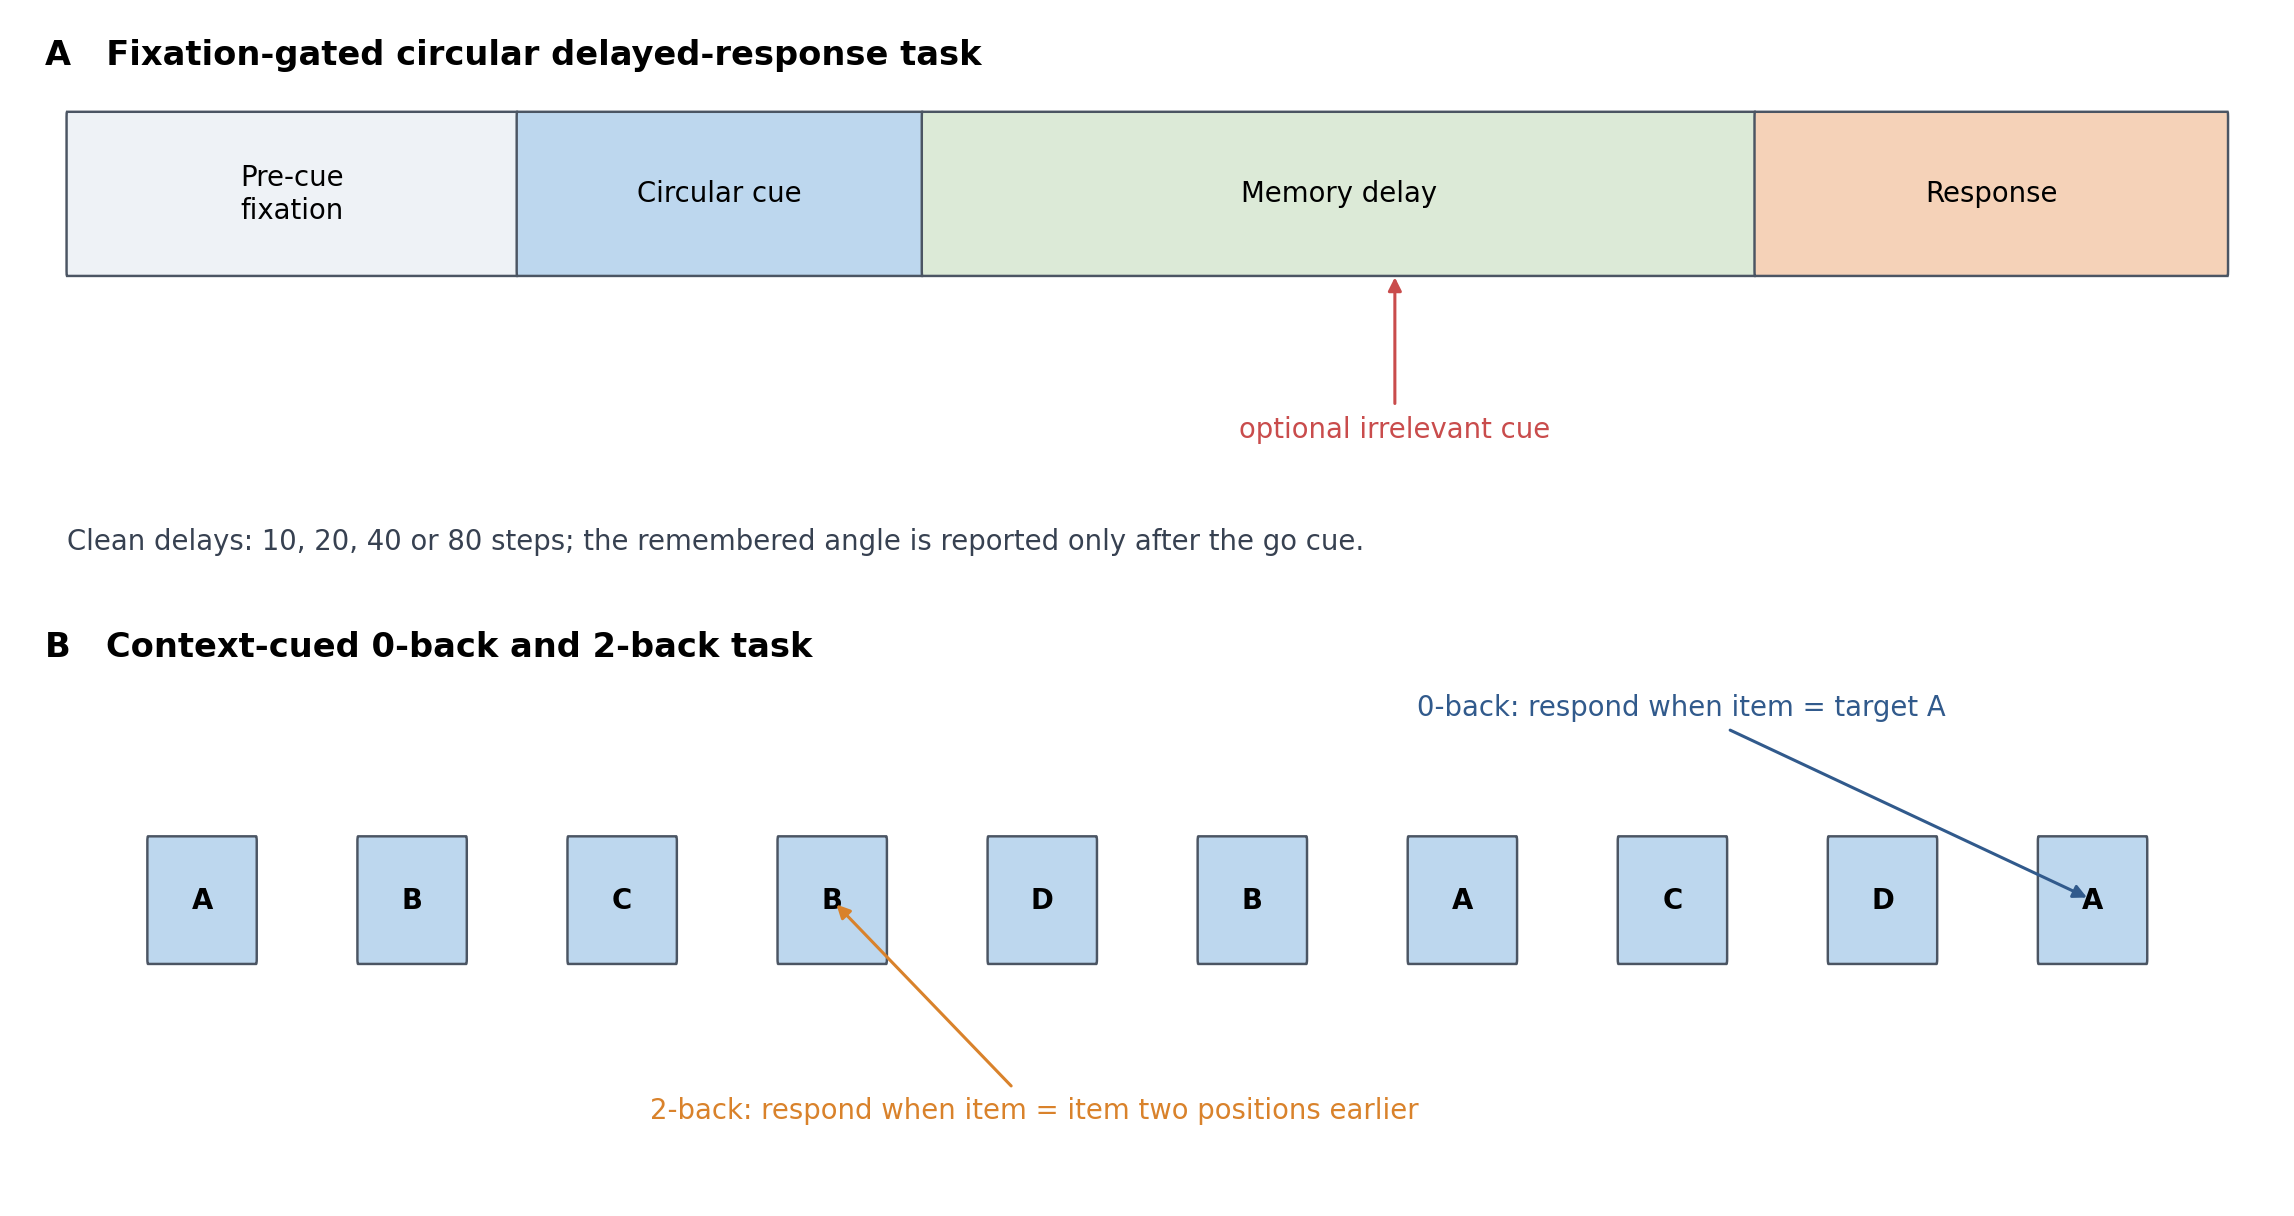
\includegraphics[width=0.98\textwidth]{task_schematic.png}
  \caption{Complementary working-memory tasks.
  \textbf{A}, The fixation-gated circular task required a continuous cue angle
  to be maintained across variable delays and reported after the go cue;
  balanced clean/distractor training made resistance to an irrelevant
  delay-period cue a learned behaviour.
  \textbf{B}, Context inputs switched the same N-back network between a
  fixed-target 0-back rule and a 2-back updating rule. The tasks supplied
  settling, delay, distractor, and updating-load contrasts rather than a single
  performance level.}
  \label{fig:tasks}
\end{figure*}

\subsection{Network architecture}

Both task families used the same rate-style continuous-time recurrent network
(CTRNN) family: a leaky recurrent hidden layer with a linear readout. The
model is not spiking, not Dale-constrained, and not intended as a
biophysically detailed cortical circuit. It is a controlled dynamical testbed
with an explicit time constant so that maintenance stability can be varied
computationally.

Let $x_t\in\mathbb{R}^{N_{\mathrm{in}}}$ be the input at discrete time $t$,
$h_t\in\mathbb{R}^{N_h}$ the hidden state, and $y_t\in\mathbb{R}^{N_{\mathrm{out}}}$
the readout. The native recurrence mixes afferent and recurrent drive,
\begin{equation}
 z_t = W_{\mathrm{in}}x_t+b_{\mathrm{in}}
      +W_{\mathrm{rec}}h_{t-1}+b_{\mathrm{rec}},
 \label{eq:drive}
\end{equation}
then applies a leaky update with nonlinearity after mixing,
\begin{equation}
 h_t = \tanh\!\left[(1-\alpha)h_{t-1}+\alpha z_t\right],
 \qquad \alpha=\frac{dt}{\tau}.
 \label{eq:native}
\end{equation}
Here $dt=20$ and $\tau=100$, so $\alpha=0.2$. The factor $(1-\alpha)$ is the
carried-state weight and $\alpha$ the drive weight. Because $\tanh$ acts after
leak mixing rather than only on $z_t$, later gain and persistence operators are
translations of this implemented update, not exact maps of a Song-style
$\tau\dot h=-h+f(z)$ form. Hidden states were initialised at zero at the start
of each trial. Outputs were a linear readout of the hidden state,
\begin{equation}
 y_t = W_{\mathrm{out}}h_t+b_{\mathrm{out}}.
 \label{eq:readout}
\end{equation}

Unless otherwise stated, $N_h=64$ and the hidden nonlinearity was $\tanh$.
The circular model used $N_{\mathrm{in}}=N_{\mathrm{out}}=33$ (32 tuned
channels plus fixation). The N-back model used eight inputs (six stimulus
identities and two rule-context channels) and two outputs (non-match and match
logits). Learned weights were frozen before all perturbation analyses.

\subsection{Training and checkpoint replication}

Throughout, a \emph{checkpoint} means one independently trained network with
frozen weights, identified by its random seed. Checkpoint, not trial or
technical replicate, is the replication unit: summary statistics are formed
across trained seeds, and within-seed trial averages are treated as
measurement precision rather than independent scientific replicates.

Circular networks were trained for 4,000 Adam updates (learning rate
$10^{-3}$, batch size 64) with Yang-style weighted fixation and response loss
on a balanced clean/distractor mixture; recurrent training noise standard
deviation was $0.05$. Six circular seeds were trained; five met preconfigured
competence limits (clean mean error $\le10^\circ$, distractor mean error
$\le15^\circ$, fixation accuracy $\ge0.90$) and were retained (seeds 20260731,
20260732, 20260733, 20260735, and 20260736). Seed 20260734 exceeded those
limits (clean $15.75^\circ$, distractor $17.46^\circ$) and was excluded before
the perturbation screen. The ten N-back checkpoints
(seeds 20260912--20260921) were drawn from a competence-screened pool trained
with staged 0-back then 2-back curriculum under Adam (learning rate $10^{-3}$,
no recurrent training noise). Final N-back retention required accuracy
$\ge0.95$, discriminability $\ge0.90$, and 2-back lure accuracy $\ge0.90$;
stage-1 0-back acquisition used stricter gates (accuracy $\ge0.98$,
discriminability $\ge0.95$).

These gates are operational competence thresholds, not fitted human effect
sizes. Chance circular error is of order $90^\circ$, so clean $\le10^\circ$
requires unambiguous angle memory while remaining softer than the few-degree
errors typical of retained seeds; distractor $\le15^\circ$ allows a modest
filtering cost without accepting near-failure. Fixation $\ge0.90$ keeps the
network in a reliable go regime so latency contrasts are not confounded by
fixation collapse. N-back gates demand near-ceiling fixed-target performance,
clearly above-chance updating, and lure resistance, so load contrasts reflect
selective updating cost rather than a weak baseline.

\subsection{Prior baseline and structured-noise background}

Earlier project stages established that continuous circular delayed response is
learnable in the same CTRNN family and that noise structure matters for
representational robustness. A categorical tanh delay baseline reached perfect
held-out accuracy across tested delays, while a tuned circular baseline
supported stable angle decoding with delay-period slowing of hidden-state
speed. Those reports remain methodological background rather than the
psilocybin-signature screen.

A five-seed structured-noise study on Yang-style fixation-gated circular
checkpoints compared matched-RMS independent Gaussian, temporal AR(1), and
topology-correlated AR(1) hidden-state noise. At equal energy, impairment
followed independent $<$ temporal $<$ topology-correlated structure, grew with
delay, accumulated during maintenance, and coincided with collapse of the
circular memory geometry. That hierarchy is retained as a robustness result
and as motivation for treating unstructured Gaussian noise as the generic
control in Section~\ref{ch:results-specificity}. Temporally persistent and
topology-aligned noise are not used as primary psychedelic candidates in the
present signature screen: they destroy representations efficiently, but they
are not the literature-preferred mechanism class for selective behavioural
dissociations.

\subsection{Candidate perturbations}

We evaluated seven single-operator families against each checkpoint's native
baseline (Table~\ref{tab:perturbations}). Operators are competing computational
interventions motivated by, but not equated with, psychedelic or working-memory
mechanisms. Because the native update applies $\tanh$ after mixing drive with
carried state, no operator is an exact biological response-gain map; each is an
explicit RNN translation. Unless noted, every non-neutral operator was applied
at every timestep of the full frozen forward pass for the entire trial or
sequence; learned weights were never updated. The only timed exception is P3b,
which is confined to the irrelevant circular-cue window. Write
$z_t^{\mathrm{w}}=W_{\mathrm{in}}x_t+W_{\mathrm{rec}}h_{t-1}$ for the
weight-derived drive. Symbols are shared across perturbations:
$x_t$ is input, $h_t$ hidden state, and $z_t$ pre-activation drive at time
$t$; $W_{\mathrm{in}}$ and $W_{\mathrm{rec}}$ are input and recurrent weights;
$b_{\mathrm{in}}$ and $b_{\mathrm{rec}}$ are biases; and $\alpha=dt/\tau$ is
the native leak factor. In P3a/P3b, $x_t^{\mathrm{stim}}$ and
$x_t^{\mathrm{ctrl}}$ denote stimulus versus fixation/rule-control channels,
with matching input submatrices $W_{\mathrm{in}}^{\mathrm{stim}}$ and
$W_{\mathrm{in}}^{\mathrm{ctrl}}$. Scalar $g$ denotes uniform gain, vector
$\mathbf{g}$ fixed unit-wise gain (P2), $\varepsilon_t\sim\mathcal{N}(0,I)$
Gaussian noise scaled by $\sigma$ (P5), $p$ persistence scale (P6), and $s$
timescale factor with derived $\alpha'$ (P7). Unless noted, learned biases
stay outside multiplicative gains.

\subsubsection{P1 Synaptic-drive gain}
Herzog et al.\ operationalised 5-HT2A effects as response gain on synaptic
current inside a nonlinearity \cite{herzog2023}; REBUS likewise links altered
precision to postsynaptic gain \cite{carhartharris2019}. In this CTRNN the
closest available analogue multiplies weight-derived drive while leaving
biases unscaled:
\begin{equation}
 h_t=\tanh\!\left[
 (1-\alpha)h_{t-1}+\alpha\bigl(g z_t^{\mathrm{w}}+b_{\mathrm{in}}+b_{\mathrm{rec}}\bigr)
 \right].
 \label{eq:p1}
\end{equation}
This is synaptic-drive gain, not an exact $F$--$I$ slope change and not a pure
carried-state manipulation.

\subsubsection{P2 Heterogeneous drive gain}
Receptor-density dependence in Herzog et al.\ implies spatially nonuniform gain
rather than one global scalar \cite{herzog2023}. We therefore replaced $g$ by a
fixed positive unit-wise vector $\mathbf{g}$ drawn from a log-normal
distribution and normalised to population mean one:
\begin{equation}
 h_t=\tanh\!\left[
 (1-\alpha)h_{t-1}+\alpha\bigl(\mathbf{g}\odot z_t^{\mathrm{w}}+b_{\mathrm{in}}+b_{\mathrm{rec}}\bigr)
 \right].
 \label{eq:p2}
\end{equation}
Three fixed vectors were treated as technical replicates and averaged within
checkpoint; they are not independent trained seeds.

\subsubsection{P3a Sensory-input gain}
REBUS predicts increased influence of afferent or bottom-up signals when
high-level precision is relaxed \cite{carhartharris2019}. As a task-level
translation, only stimulus-channel input weights were scaled, leaving fixation
or rule-context channels unchanged:
\begin{equation}
\begin{aligned}
 z_t^{\mathrm{in}} &=
 g\,W_{\mathrm{in}}^{\mathrm{stim}}x_t^{\mathrm{stim}}
 +W_{\mathrm{in}}^{\mathrm{ctrl}}x_t^{\mathrm{ctrl}}
 +b_{\mathrm{in}},\\
 h_t &= \tanh\bigl[(1-\alpha)h_{t-1}
 +\alpha(z_t^{\mathrm{in}}+W_{\mathrm{rec}}h_{t-1}+b_{\mathrm{rec}})\bigr].
\end{aligned}
 \label{eq:p3a}
\end{equation}
This tests sensory sensitivity, not receptor-mapped response gain.

\subsubsection{P3b Distractor-window gain}
Human psilocybin work shows particular vulnerability when competing information
must be ignored \cite{carter2005}. P3b applies Eq.~\eqref{eq:p3a} only during
the irrelevant circular cue and is therefore a circular-task manipulation
check rather than a complete cross-task mechanism candidate.

\subsubsection{P4 Recurrent gain}
Recurrent excitation is a canonical substrate of delay-period maintenance
\cite{wang2013nmda}. To separate recurrent weighting from sensory drive we
scaled only the recurrent weight contribution:
\begin{equation}
\begin{aligned}
 z_t^{(4)} &=
 W_{\mathrm{in}}x_t+b_{\mathrm{in}}
 +g W_{\mathrm{rec}}h_{t-1}+b_{\mathrm{rec}},\\
 h_t &= \tanh\bigl[(1-\alpha)h_{t-1}+\alpha z_t^{(4)}\bigr].
\end{aligned}
 \label{eq:p4}
\end{equation}
Recurrent bias remained outside the gain. P4 is a mechanistic contrast within
the trained RNN, not a direct REBUS or 5-HT2A claim.

\subsubsection{P5 Gaussian state noise}
Independent Gaussian noise is retained in the project catalogue as a generic
disruption control against which selective signatures must later be shown to
exceed nonspecific damage. Noise was added to the pre-activation,
\begin{equation}
 h_t=\tanh\!\left[
 (1-\alpha)h_{t-1}+\alpha z_t+\sigma\varepsilon_t
 \right],
 \quad \varepsilon_t\sim\mathcal{N}(0,I),
 \label{eq:p5}
\end{equation}
in the exploratory pilot, but P5 was outside the candidate-only screen reported
in Section~\ref{ch:results-screen}. Section~\ref{ch:results-specificity} is
reserved for the matched-cost comparison.

\subsubsection{P6 State persistence}
Trained working-memory RNNs can store information in slow or persistent latent
dynamics \cite{ghazizadeh2021,wang2013nmda}. P6 asks whether weakening
retention of the carried state, without rescaling incoming drive, can produce
selective behavioural costs. The update is asymmetric:
\begin{equation}
 h_t=\tanh\!\left[p(1-\alpha)h_{t-1}+\alpha z_t\right],
 \label{eq:persistence}
\end{equation}
where $p$ is the persistence scale. This is an operational RNN intervention,
not a pre-specified biological mapping from psilocybin to reduced persistence;
$p=0.95$ entered the present screen as the exploratory pilot nominee.

\subsubsection{P7 Conserved effective time constant}
To test whether P6 effects are merely those of any timescale change, P7
rescales the leaky-integrator coefficients while preserving their sum. With
timescale factor $s$,
\begin{equation}
 \alpha'=\min(\alpha/s,1),\qquad
 h_t=\tanh\!\left[(1-\alpha')h_{t-1}+\alpha'z_t\right].
 \label{eq:p7}
\end{equation}
Thus $s>1$ slows the effective timescale and $s<1$ speeds it. Within the
evaluated grid, $\alpha/s<1$, so the minimum was inactive. P7 is a
mechanistic control for conserved timescale change, not a psychedelic
parameter claim.

\begin{table*}[t]
\caption{Candidate perturbations and fixed evaluation grids.
Neutral settings reproduce the native forward pass. Distractor-window gain was
defined only for the circular distractor condition; all other operators except
P5 were evaluated in both task families. P5 is listed for catalogue continuity
but was not part of the candidate-only screen.}
\label{tab:perturbations}
\centering
\begin{tabular}{lll}
\toprule
ID & Computational intervention & Strengths \\
\midrule
P1 & Scalar gain on input and recurrent weight drive
& 0.90--1.10 \\
P2 & Fixed mean-one unit-wise log-normal gain
& log-SD 0.00--0.30 \\
P3a & Gain on stimulus-channel input contribution
& 0.80--1.20 \\
P3b & P3a restricted to irrelevant cue window
& 1.00--1.50 \\
P4 & Scalar gain on recurrent weight contribution
& 0.90--1.10 \\
P5 & Additive pre-activation noise (catalogue)
& specificity chapter \\
P6 & Scale $p$ on carried-state coefficient
& 0.90--1.10 \\
P7 & Conserved update with $\alpha'=\min(\alpha/s,1)$
& 0.80--1.25 \\
\bottomrule
\end{tabular}
\end{table*}

\subsection{Evaluation and behavioural signature}

Each circular checkpoint, operator, strength, condition, and delay used 1,024
trials. Each N-back checkpoint, operator, strength, and load used 1,024
20-item sequences. Native and perturbed evaluations reused identical generated
task samples within checkpoint and cell.

Circular response accuracy was mean absolute angular error. Post-cue settling
was the first response step at which angular error was below $15^\circ$ and
population-vector amplitude exceeded 50\% of the native reference amplitude.
Trials that did not settle were capped at the 25-step response duration,
yielding restricted mean settling time. Settling was interpreted only when
fixation accuracy was at least 0.90 and at least 80\% of trials settled.
The $15^\circ$ settling threshold is a coarse latency criterion distinct from
continuous accuracy; half-native amplitude excludes collapsed bumps; and the
80\% settled floor marks latency invalid when most trials never settle.
``Slowing with preservation'' required a positive settling change at clean
delay 20 while proportional angular-error impairment remained at or below
0.20, encoding selective slowing without large accuracy loss.

For circular condition $c$, proportional impairment was
\begin{equation}
 I_c=\frac{E_{\mathrm{perturbed},c}-E_{\mathrm{native},c}}
 {E_{\mathrm{native},c}},
\end{equation}
where $E$ is mean angular error. Delay selectivity was
$I_{\mathrm{delay\,80}}-I_{\mathrm{delay\,10}}$; distractor selectivity was
$I_{\mathrm{distractor\,20}}-I_{\mathrm{clean\,20}}$.

N-back discriminability was $D=H-F$, where $H$ and $F$ are hit and false-alarm
rates. Condition-normalised impairment was
\begin{equation}
 J_c=\frac{D_{\mathrm{native},c}-D_{\mathrm{perturbed},c}}
 {D_{\mathrm{native},c}},
\end{equation}
and load selectivity was $J_{\mathrm{2back}}-J_{\mathrm{0back}}$. Positive
values indicate disproportionate high-load impairment.

The candidate-screen analysis was descriptive. For each operator-strength
setting we reported the checkpoint mean, SD, and a student $t$ 95\% interval
across seeds, together with the fraction of seeds in the predicted direction.
A setting met the complete descriptive pattern when the mean
slowing-with-preservation, distractor, and N-back load contrasts were positive
and at least a simple majority of checkpoints agreed on each (three of five
circular; six of ten N-back); delay selectivity was supporting evidence only.
That majority rule generalises the exploratory pilot's $\ge$2-of-3 criterion
and is implemented in the summary code; it was not restated as a numeric
threshold in the 1,024-trial preregistration text. Cross-operator comparisons
are uncontrolled for overall perturbation magnitude, so a near-miss may fail
because of dose as well as mechanism. No participant-level inference,
confirmatory $p$ values, or multiple-comparison claims were made for the
screen.

\section{Results: Baseline Competence and Hidden-State Geometry}
\label{ch:results-baseline}

Before comparing perturbations, the retained circular and N-back checkpoints
must be competent on their native tasks and must exhibit interpretable
hidden-state organisation. This section reports those baselines. Pool
competence uses the frozen held-out banks already recorded at screening;
delay-sweep and dynamics panels use representative retained seeds
(circular seed 20260735; N-back seed 20260916).

\subsection{Distractor-trained circular baselines}

Across the five retained distractor-trained circular checkpoints, held-out
mean angular error averaged $2.70^\circ$ on clean delay-20 trials and
$3.54^\circ$ with a mid-delay distractor (Fig.~\ref{fig:baseline-circular-competence}).
All retained seeds passed the preconfigured competence gates (clean
$\le10^\circ$, distractor $\le15^\circ$, fixation accuracy $\ge0.90$). Seed
20260734 failed those gates and was excluded before the perturbation screen;
it is shaded in the pool figure for transparency.

\begin{figure*}[t]
  \centering
  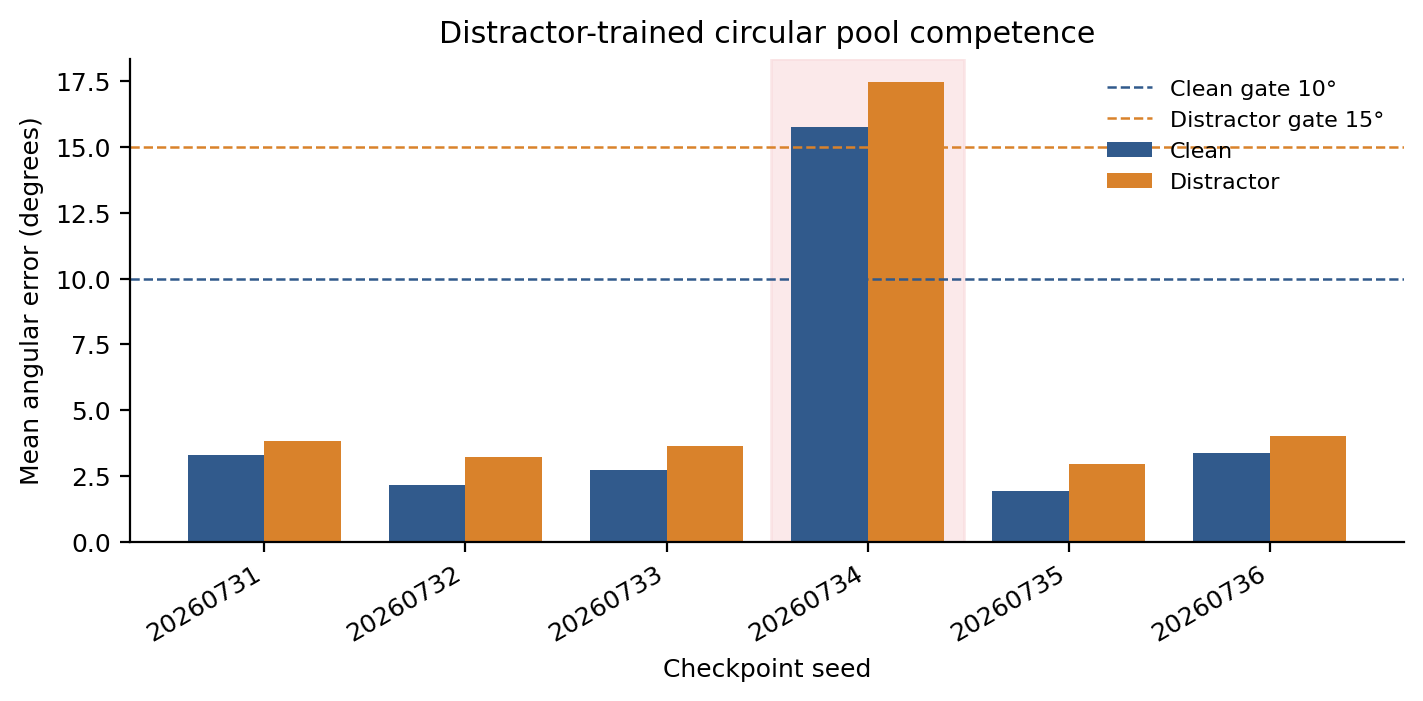
\includegraphics[width=0.92\textwidth]{circular_trained_distractor_pool_competence.png}
  \caption{Clean versus distractor mean angular error for every trained
  circular seed. Retained checkpoints lie well below the competence gates;
  the failed seed is shaded.}
  \label{fig:baseline-circular-competence}
\end{figure*}

On the representative retained seed, clean mean error rose only gradually
with delay ($1.71^\circ$, $1.86^\circ$, $2.10^\circ$, and $2.61^\circ$ at delays
10, 20, 40, and 80), while the distractor delay-20 cell remained low at
$2.92^\circ$ (Fig.~\ref{fig:baseline-circular-delay}). Hidden-state PCA
showed angle-ordered trajectories occupying a ring-like plane
(Fig.~\ref{fig:baseline-circular-dynamics}A; PC1+PC2 $=70.4\%$ variance).
Step-to-step hidden-state speed slowed during the silent delay
(Fig.~\ref{fig:baseline-circular-dynamics}B), and a ridge decoder fit on
delay-period hidden states recovered cue angle with mean delay error
$0.41^\circ$ (Fig.~\ref{fig:baseline-circular-dynamics}C). Because the
fixation-gated population readout is trained to remain silent until the go
cue, that decoder is a hidden-state diagnostic rather than the behavioural
output itself.

\begin{figure*}[t]
  \centering
  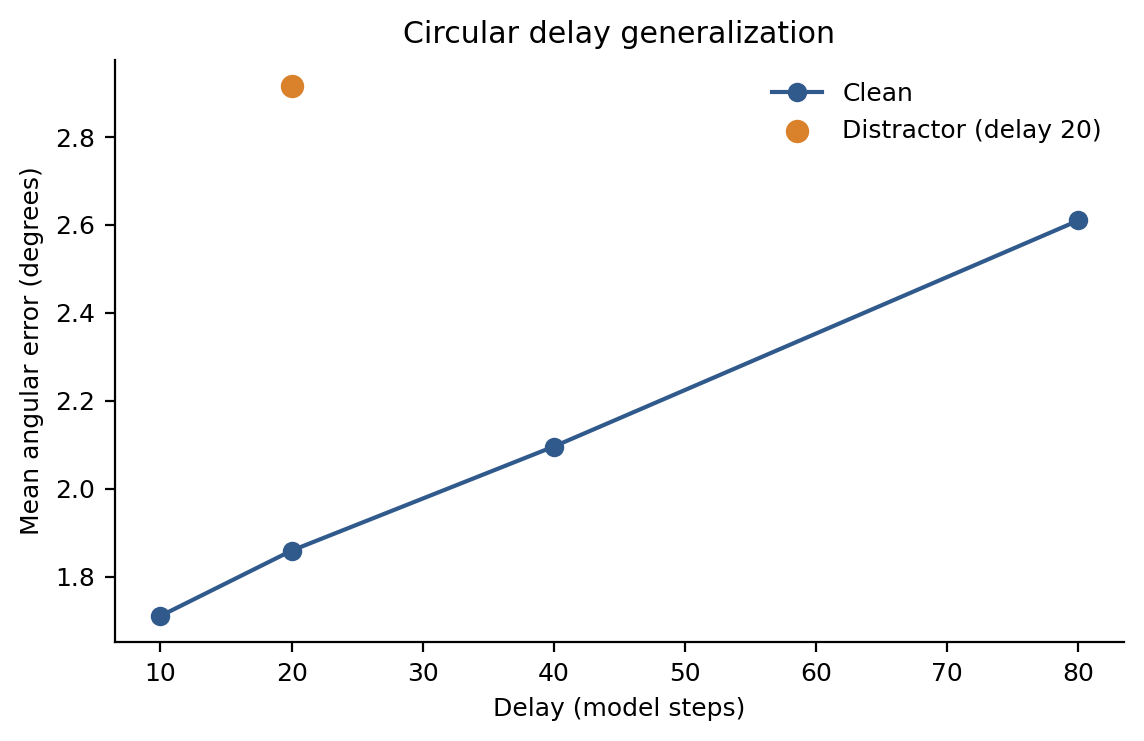
\includegraphics[width=0.55\textwidth]{circular_trained_distractor_delay_sweep.png}
  \caption{Clean delay generalization for representative circular seed
  20260735, with the distractor delay-20 cell marked separately.}
  \label{fig:baseline-circular-delay}
\end{figure*}

\begin{figure*}[t]
  \centering
  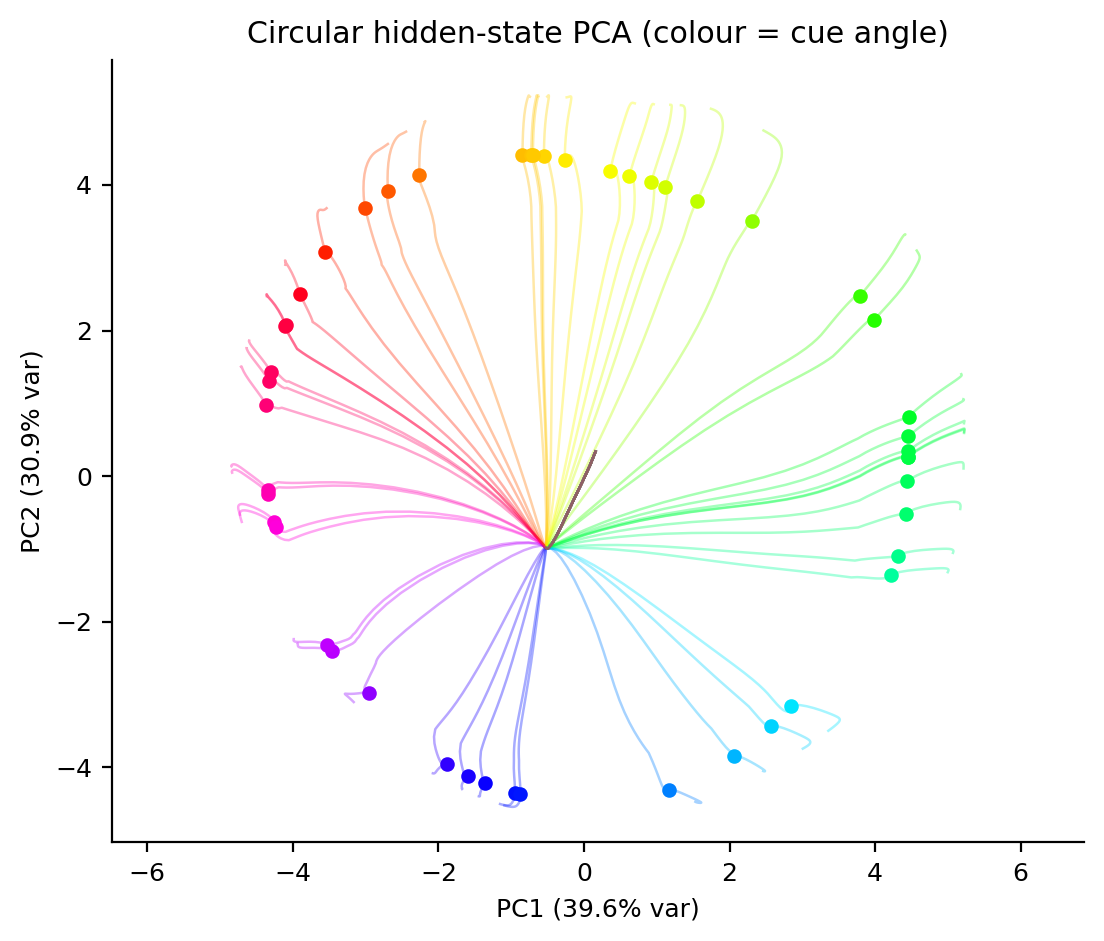
\includegraphics[width=0.32\textwidth]{circular_trained_distractor_pca_trajectories.png}\hfill
  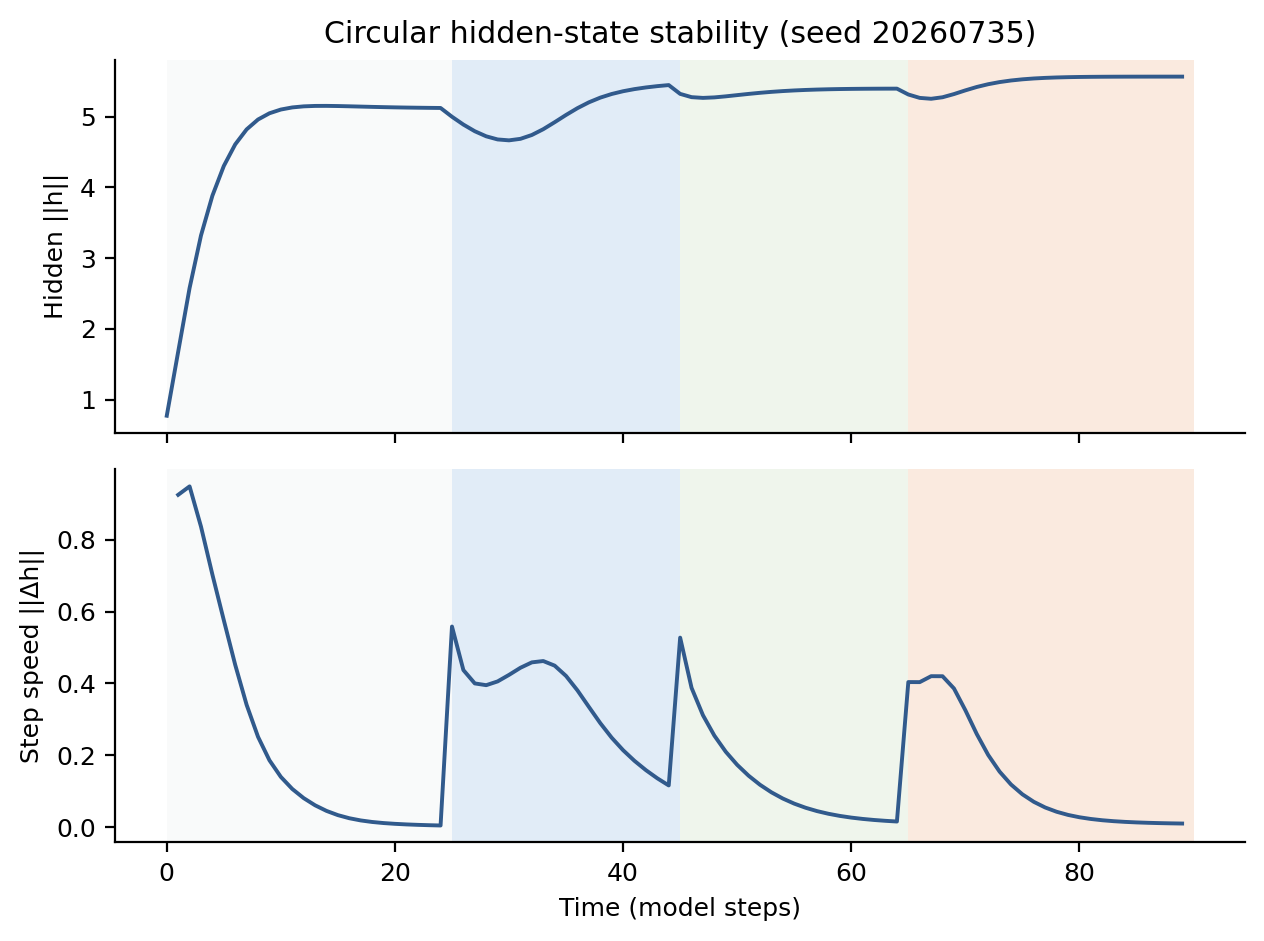
\includegraphics[width=0.32\textwidth]{circular_trained_distractor_stability.png}\hfill
  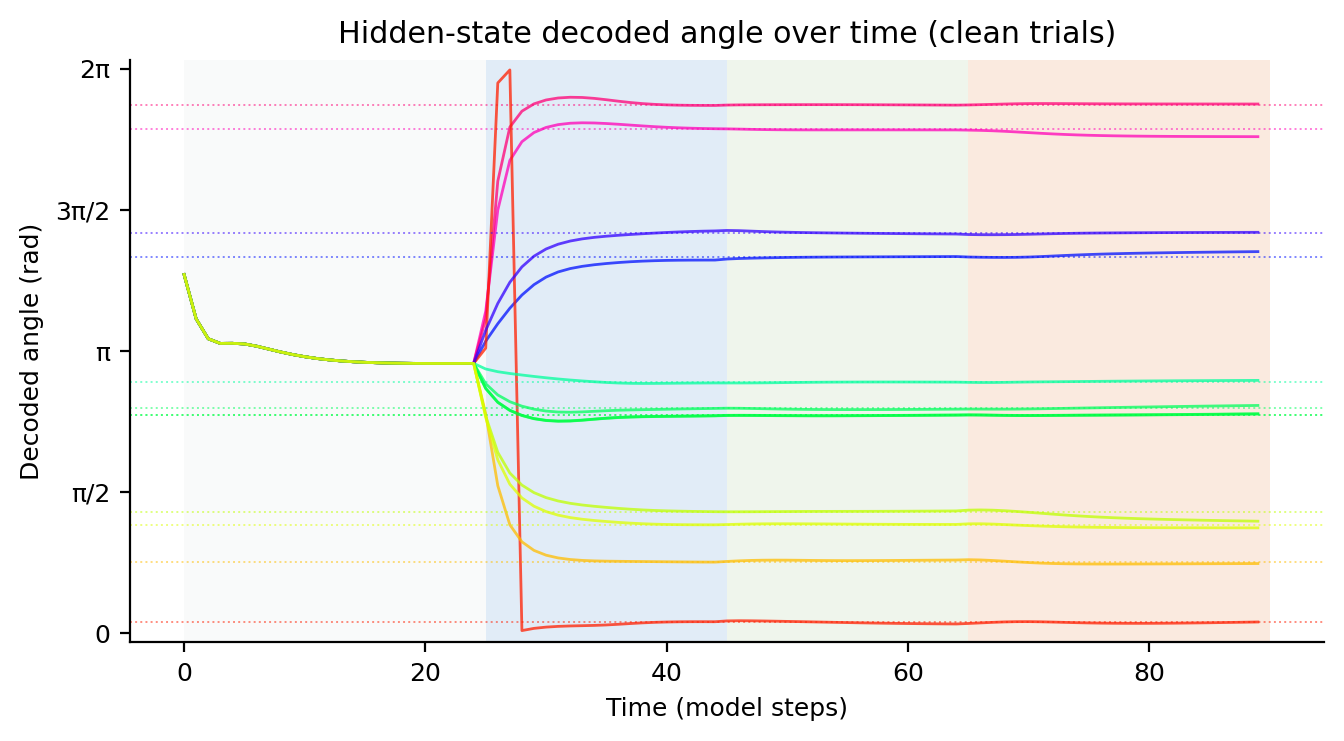
\includegraphics[width=0.32\textwidth]{circular_trained_distractor_decoded_angle_over_time.png}
  \caption{Circular hidden-state organisation on seed 20260735.
  \textbf{A}, PCA trajectories coloured by cue angle.
  \textbf{B}, Hidden-state norm and step speed across trial phases.
  \textbf{C}, Hidden-state decoded angle over time on clean trials.}
  \label{fig:baseline-circular-dynamics}
\end{figure*}

\subsection{Competence-screened N-back baselines}

All ten screened N-back checkpoints passed untouched competence gates
(Fig.~\ref{fig:baseline-nback-competence}). 0-back accuracy was at ceiling
in every seed; 2-back accuracy ranged from $0.958$ to $0.986$, with
discriminability (hit rate minus false-alarm rate) from $0.917$ to $0.971$
and 2-back lure accuracy from $0.964$ to $0.996$. On representative seed
20260916, the frozen evaluation bank gave 0-back accuracy/discriminability
of $1.000$ and 2-back values of $0.986$/$0.971$
(Fig.~\ref{fig:baseline-nback-load}).

\begin{figure*}[t]
  \centering
  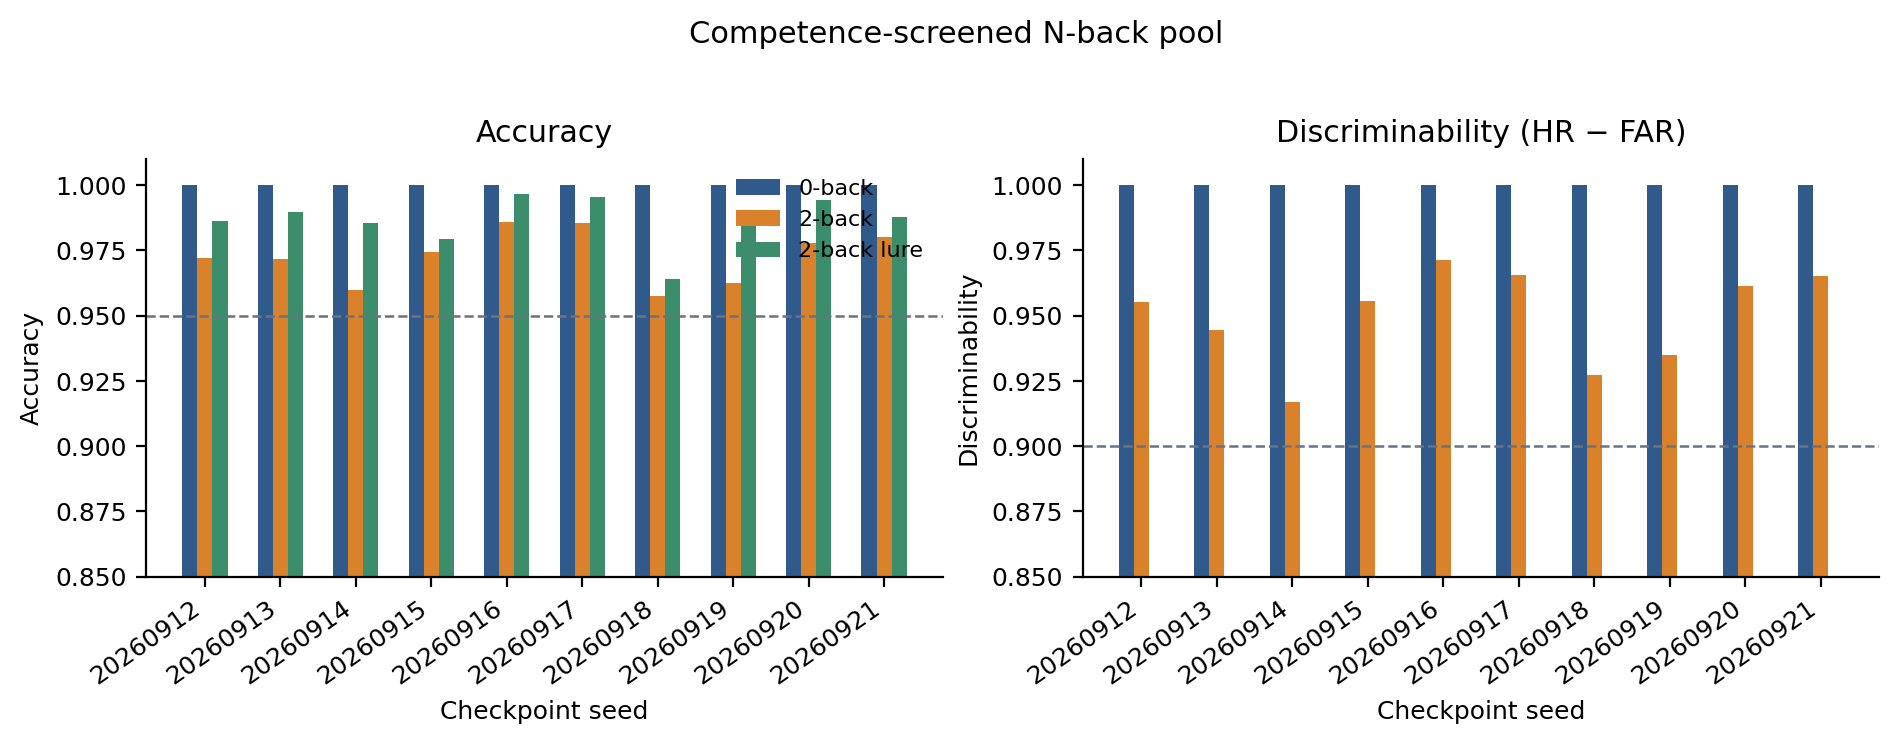
\includegraphics[width=0.92\textwidth]{nback_screened_pool_competence.png}
  \caption{0-back versus 2-back accuracy, discriminability, and 2-back lure
  accuracy across the ten retained N-back checkpoints.}
  \label{fig:baseline-nback-competence}
\end{figure*}

\begin{figure*}[t]
  \centering
  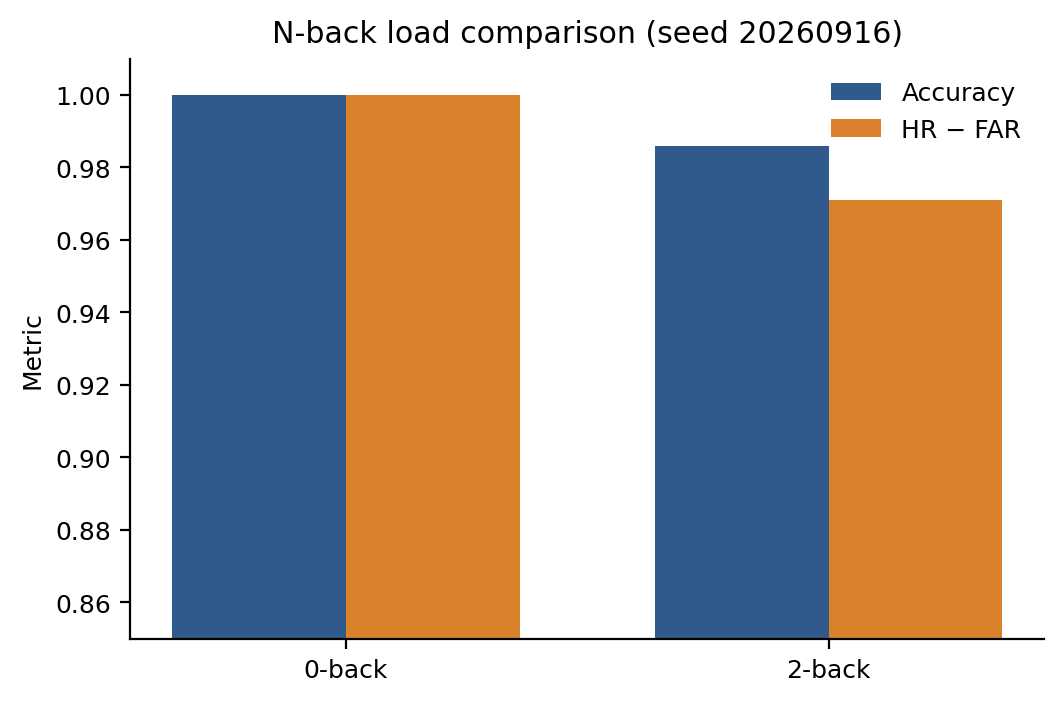
\includegraphics[width=0.48\textwidth]{nback_screened_load_comparison.png}
  \caption{Representative N-back load comparison on seed 20260916 under the
  frozen evaluation bank.}
  \label{fig:baseline-nback-load}
\end{figure*}

Hidden-state geometry differed by rule (Fig.~\ref{fig:baseline-nback-dynamics}A).
At stimulus samples, 0-back activity formed tight clusters by current
stimulus identity, whereas 2-back geometry was more overlapping, consistent
with an updating demand that cannot be solved from the current item alone.
Hidden-state speed under 2-back remained phasic across the sequence
(Fig.~\ref{fig:baseline-nback-dynamics}B). Match probability for scored
2-back items separated match from non-match events within each item window
(Fig.~\ref{fig:baseline-nback-dynamics}C).

\begin{figure*}[t]
  \centering
  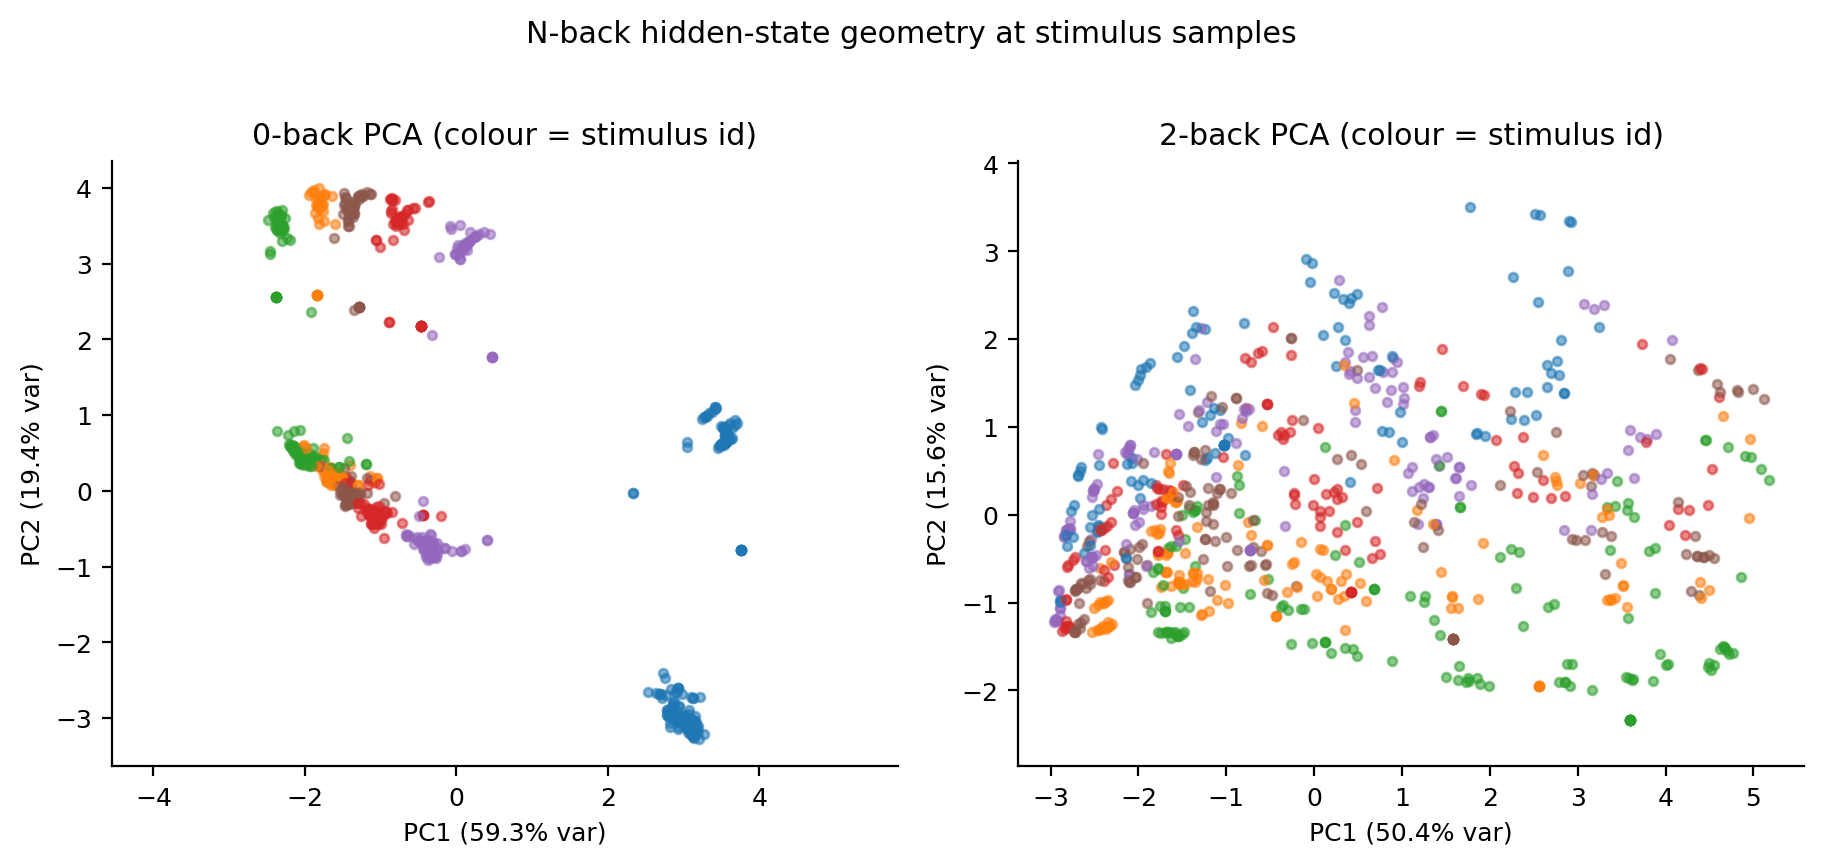
\includegraphics[width=0.32\textwidth]{nback_screened_pca_trajectories.png}\hfill
  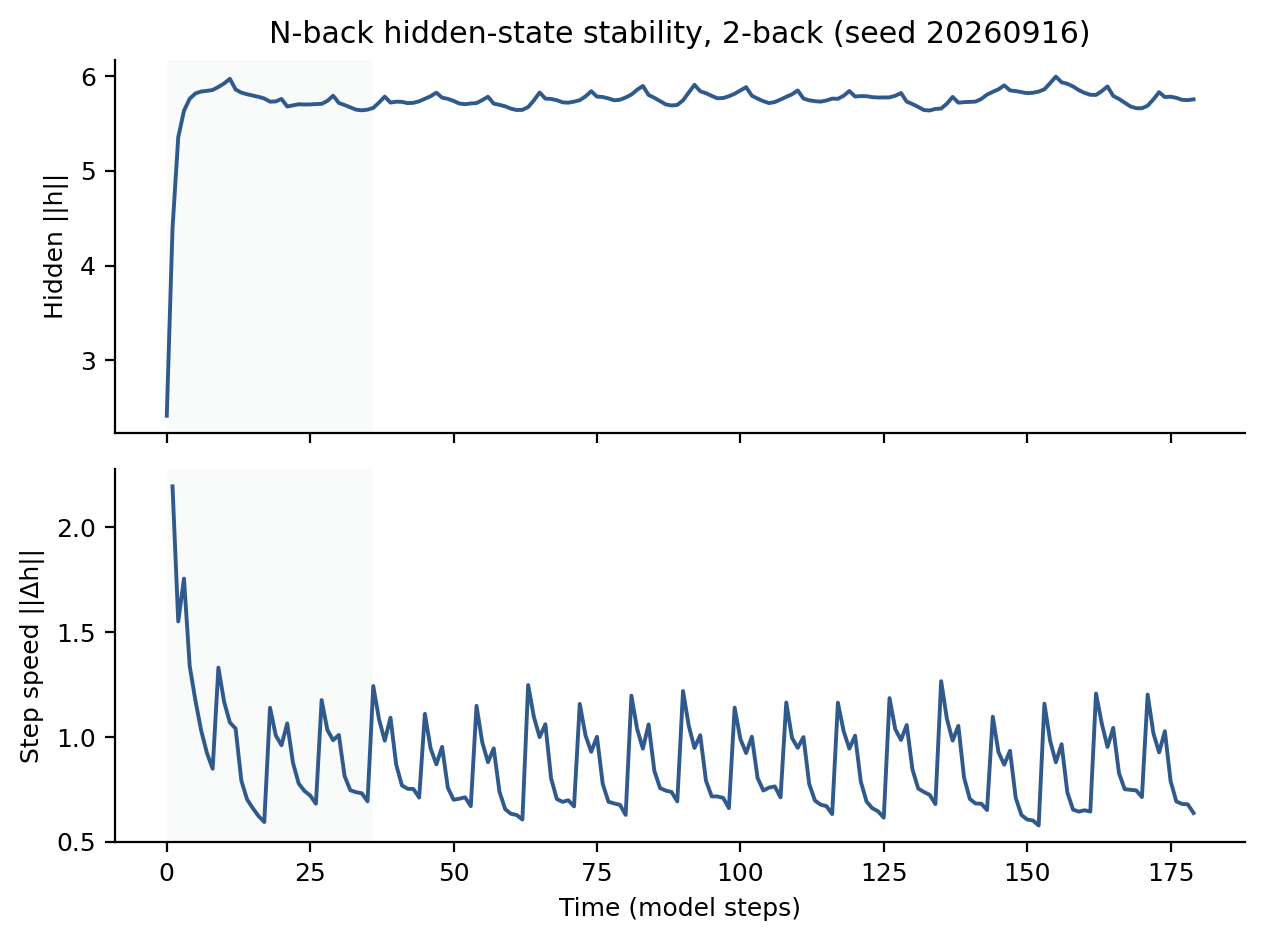
\includegraphics[width=0.32\textwidth]{nback_screened_stability.png}\hfill
  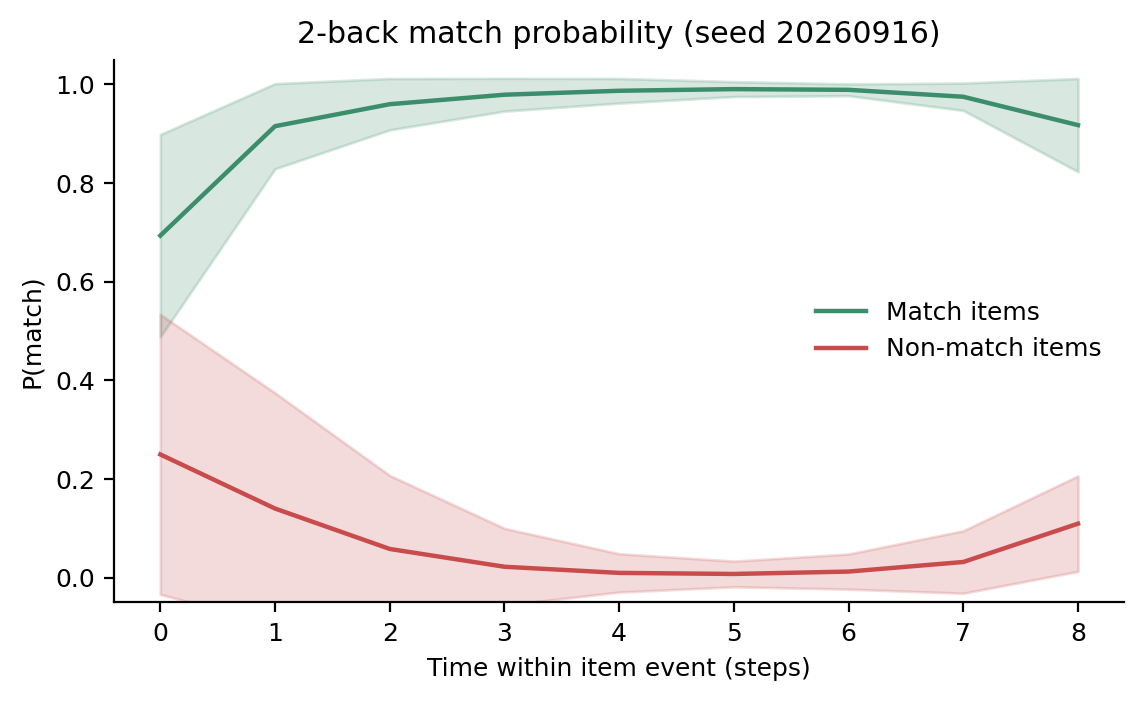
\includegraphics[width=0.32\textwidth]{nback_screened_match_probability.png}
  \caption{N-back hidden-state organisation on seed 20260916.
  \textbf{A}, PCA at stimulus samples coloured by stimulus identity under
  0-back and 2-back rules.
  \textbf{B}, Hidden-state norm and step speed during 2-back sequences.
  \textbf{C}, Mean match probability for match versus non-match scored items.}
  \label{fig:baseline-nback-dynamics}
\end{figure*}

These baselines establish that both families solve their native tasks with
interpretable internal structure before any literature-motivated
perturbation is applied.

\section{Results I: Candidate Perturbation Screen}
\label{ch:results-screen}

This section reports the completed candidate-versus-native-baseline screen.
It nominates a leading operator but does not yet establish specificity against
generic damage.

\subsection{Nomination and independent circular retest isolated one complete profile}

State persistence $0.95$ was first nominated by an exploratory three-seed pilot
on an earlier circular family without trained distractors. The present screen
retested all candidate strengths on the new distractor-trained circular family
and reused the completed ten-checkpoint N-back grid. Across the 23 non-neutral
shared operator-strength profiles, only persistence $0.95$ again met the
complete descriptive majority pattern (Fig.~\ref{fig:screen}). It showed
slowing with preservation, long-delay selectivity, and distractor selectivity
in four of five circular checkpoints, together with load selectivity in all
ten N-back checkpoints. Relative to the pilot, circular delay selectivity
shrank from $0.290$ to $0.089$ and distractor selectivity from $0.148$ to
$0.015$, while N-back load selectivity remained similar ($0.296$ to $0.250$).
Neutral settings returned zero contrast. Other perturbations often reproduced
one or two components, but not the full combination.

\begin{figure*}[t]
  \centering
  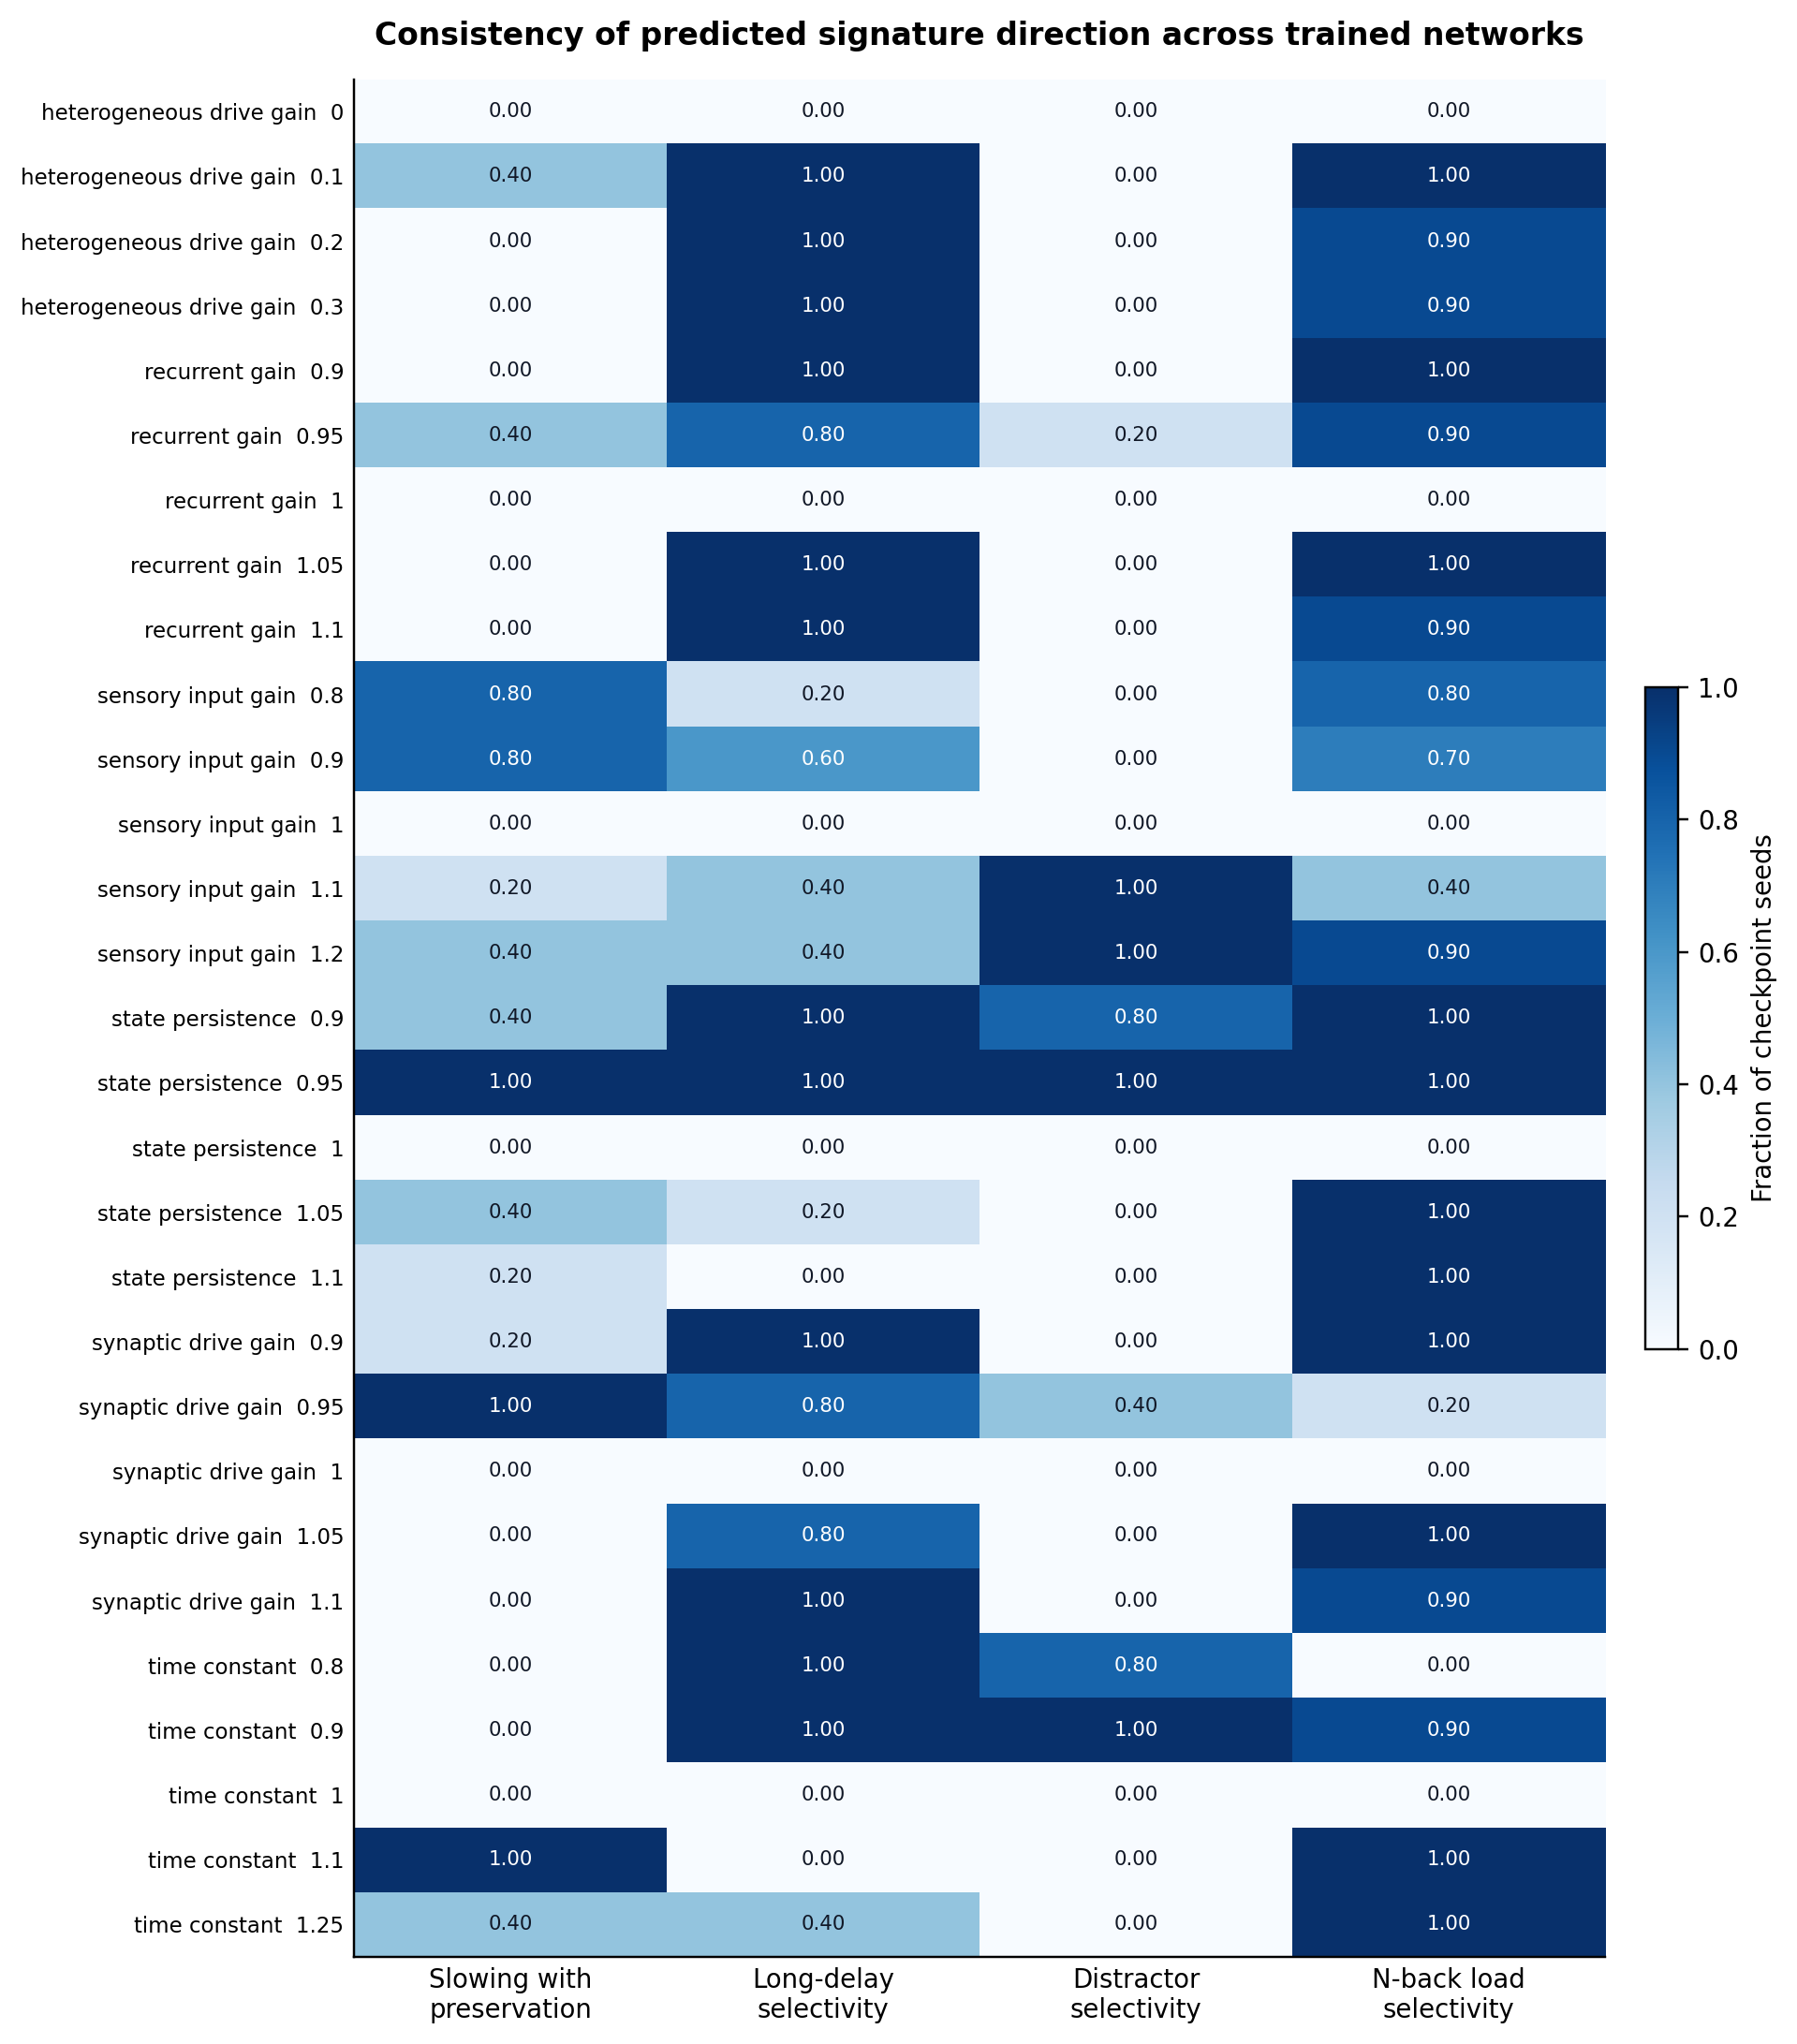
\includegraphics[height=0.70\textheight]{signature_screen.png}
  \caption{Cross-task signature screen.
  Rows are every shared operator-strength setting evaluated in both task
  families; columns show the fraction of independent checkpoint seeds with the
  predicted signature direction. Circular fractions have denominator five and
  N-back fractions denominator ten. State persistence 0.95 was the only row to
  meet the complete majority pattern and additionally reached 4/5 agreement on
  each circular feature with complete N-back agreement. Values quantify
  directional consistency, not participant-level probability or statistical
  significance.}
  \label{fig:screen}
\end{figure*}

\subsection{A 5\% persistence reduction preserved ordinary accuracy while
selectively affecting demanding conditions}

At $p=0.95$, clean delay-20 proportional angular-error change was
$0.049\pm0.092$ across circular checkpoints (95\% $t$-interval
$[-0.065,0.164]$) and remained below $0.20$ in 5/5 seeds. Restricted mean
settling increased by $0.104\pm0.167$ steps ($[-0.103,0.312]$) and was
positive in 4/5 seeds, with a range of $-0.013$ to $0.393$ steps
(Table~\ref{tab:leading}). The circular settling, delay, and distractor
intervals all include zero, so those components are directional majority
tendencies rather than robust across-checkpoint effects. By contrast, N-back
load selectivity was $0.250\pm0.077$ ($[0.195,0.305]$), positive in 10/10
checkpoints, and ranged from $0.110$ to $0.363$. Long-minus-short delay
selectivity was $0.089\pm0.075$ ($[-0.004,0.181]$) and distractor-minus-clean
selectivity was $0.015\pm0.044$ ($[-0.040,0.071]$), each positive in 4/5
checkpoints. Thus the leading perturbation retained the predicted average
ordering, but only the N-back contrast clearly excluded zero under the
seed-level $t$-interval.

\begin{table*}[t]
\caption{State persistence 0.95. Values are mean $\pm$ SD across five
circular or ten N-back checkpoint seeds; intervals are student $t$ 95\%
intervals across those seeds.}
\label{tab:leading}
\centering
\begin{tabular}{lccc}
\toprule
Outcome & Contrast & 95\% interval & Consistency \\
\midrule
Delay-20 error & $0.049\pm0.092$ & $[-0.065,0.164]$ & below 0.20 in 5/5 \\
Settling change (steps) & $0.104\pm0.167$ & $[-0.103,0.312]$ & 4/5 positive \\
Delay selectivity & $0.089\pm0.075$ & $[-0.004,0.181]$ & 4/5 positive \\
Distractor selectivity & $0.015\pm0.044$ & $[-0.040,0.071]$ & 4/5 positive \\
N-back load selectivity & $0.250\pm0.077$ & $[0.195,0.305]$ & 10/10 positive \\
\bottomrule
\end{tabular}
\end{table*}

\subsection{The persistence effect was dose-like but not monotonic across all
features}

Reducing persistence further to 0.90 enlarged mean settling, delay, and N-back
load effects (Fig.~\ref{fig:persistence}). However, slowing with preservation
passed only 1/5 circular checkpoints, so the stronger intervention no longer
expressed the selective accuracy-preserving pattern. Increasing persistence
above one continued to impair N-back preferentially but reversed the circular
delay and distractor contrasts. The joint signature was therefore specific to
a weak reduction around 0.95 rather than monotonic damage at any non-neutral
strength.

\begin{figure*}[t]
  \centering
  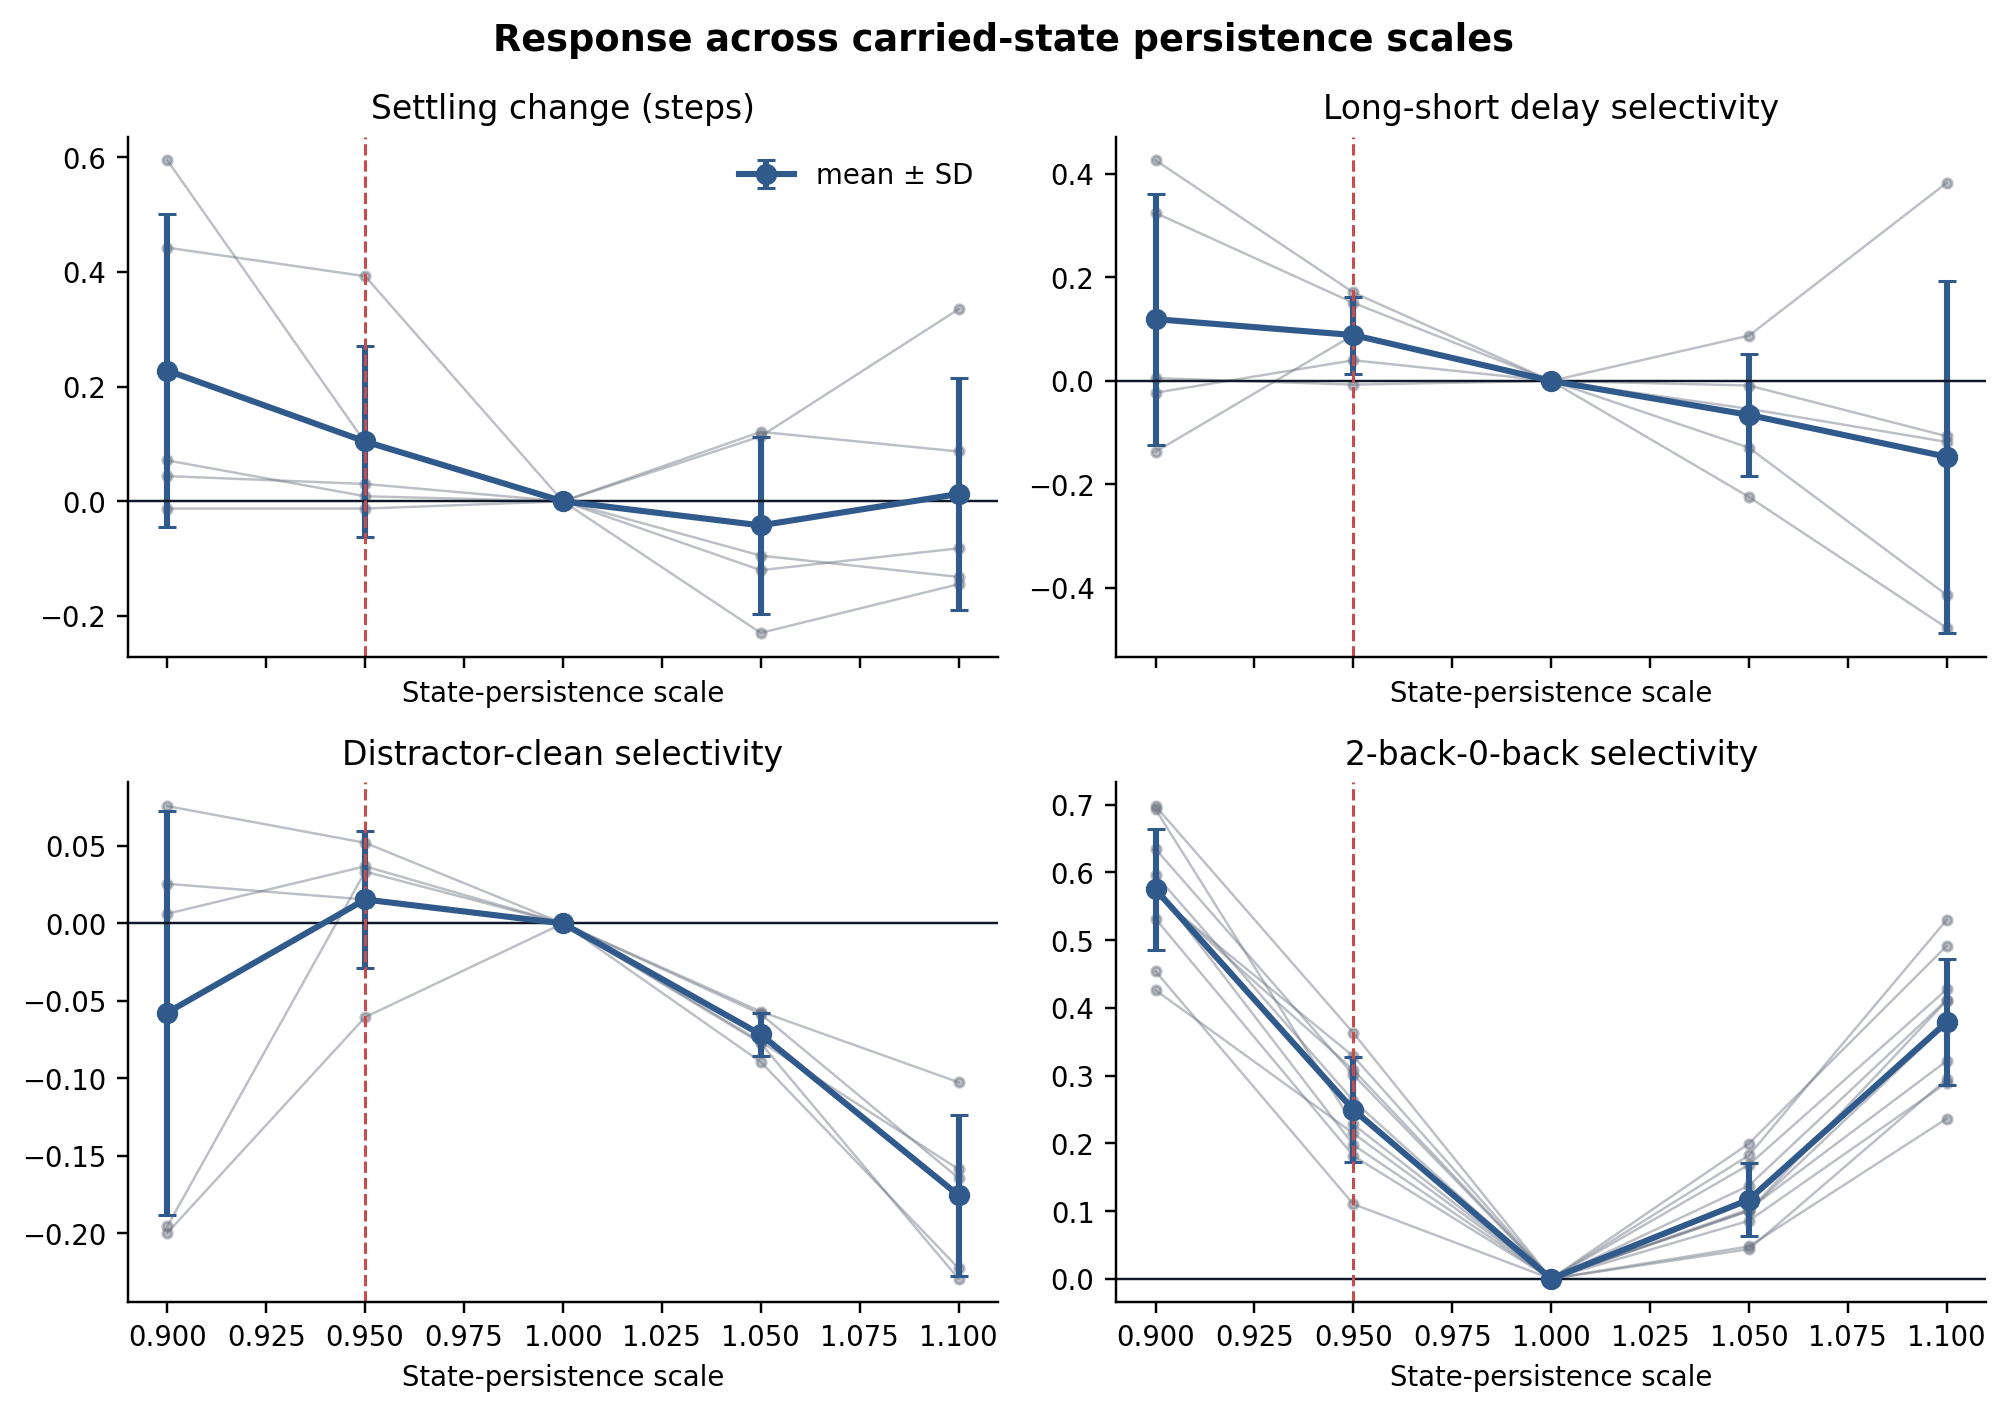
\includegraphics[width=0.98\textwidth]{persistence_dose_response.png}
  \caption{Dose-like response to carried-state persistence scaling.
  Grey lines are independently trained checkpoint seeds; blue points and error
  bars are mean $\pm$ SD. The dashed red line marks the leading scale 0.95 and
  the horizontal line marks no change from native performance. A stronger
  reduction increased several impairments but also violated relative
  preservation, whereas increased persistence reversed circular delay and
  distractor selectivity.}
  \label{fig:persistence}
\end{figure*}

\subsection{Alternative operators reproduced partial signatures}

Sensory-input gain 1.20 produced distractor selectivity in 5/5 circular
checkpoints and load selectivity in 9/10 N-back checkpoints, but mean settling
became slightly faster ($-0.010\pm0.023$ steps; positive in only 1/5) and delay
selectivity was positive in only 1/5. Effective time-constant scale 1.10 slowed
settling with preservation in 5/5 ($0.605\pm0.176$ steps) and showed load
selectivity in 10/10, but distractor selectivity was negative in every circular
checkpoint. Conversely, time-constant scale 0.90 showed delay selectivity in
5/5 and distractor selectivity in 4/5 but accelerated settling in every
circular checkpoint ($-0.681\pm0.170$ steps). Synaptic-drive gain 1.05 showed
delay selectivity in 4/5, distractor selectivity in 3/5, and load selectivity
in 10/10, but also accelerated settling in 5/5 ($-0.496\pm0.240$ steps). All of
these near-miss clean delay-20 settling cells were latency-valid; uniqueness
was therefore not an artefact of invalid latency scoring. These near-misses
constrain the result: matching one difficult condition was insufficient to
qualify as the complete pattern, and the discrimination against the conserved
time-constant operator rested on settling direction and distractor selectivity
rather than on large absolute settling magnitude.

The contrast between persistence and the conserved time-constant operator is
mechanistically informative. Both reduced persistence ($p<1$) and reduced
timescale ($s<1$) can weaken retention, but only persistence leaves the drive
coefficient unchanged (Eq.~\ref{eq:persistence}). Reducing the conserved
timescale ($s=0.90$) accelerated post-cue settling while preserving delay and
distractor selectivity; increasing it ($s=1.10$) slowed settling but reversed
distractor selectivity. The joint pattern therefore depended on the asymmetric
carried-state intervention, not merely on any reduction in effective memory
lifetime. Cross-operator comparisons remain uncontrolled for overall clean-task
cost, so dose differences could still contribute to some near-misses.

\subsection{Trained distractor filtering resolved the prior validity failure}

All 945 circular result rows passed the fixation gate, all ten N-back native
checkpoints passed competence, and all $p=0.95$ clean delay-20 cells were
latency-valid. Twelve rows elsewhere in the circular grid were latency-invalid
(all heterogeneous-drive settings with low settled fraction); none of the
near-miss settling comparisons above used those cells. Native distractor mean
error now ranged from $3.46^\circ$ to $4.83^\circ$, and every native distractor
cell had a settled fraction of 1.00. The distractor contrast therefore measured
perturbation of a learned filtering behaviour rather than failure on an
unfamiliar task. As a manipulation check, distractor-window gains 1.10, 1.25,
and 1.50 increased distractor error by 3.7\%, 9.8\%, and 21.5\% on average,
respectively, with positive effects in 5/5 checkpoints. However,
persistence-related distractor selectivity remained small and was negative in
one checkpoint, so the improved validity does not convert the result into a
strong human effect-size match.

A three-seed exploratory pilot had already suggested that persistence $0.95$
can exceed weak Gaussian state noise on N-back load selectivity at nearly
matched 0-back cost (means $0.296$ versus $0.052$ at noise SD $0.025$). That
observation is labelled secondary, used only three N-back checkpoints, and did
not yield an informative circular cost match within the pilot's $0.05$
tolerance; it is therefore not a specificity claim for the present screen.

\section{Results II: Specificity Against Generic Disruption}
\label{ch:results-specificity}

\begin{scaffold}
This section is required by the dissertation end goal and is not yet written.
Intended content:
\begin{itemize}[leftmargin=*]
  \item Pre-register persistence $0.95$ versus matched-cost Gaussian state
        noise (P5) on the trained-distractor circular family and the
        competence-screened N-back family.
  \item Match on clean-task proportional cost before comparing excess
        settling, delay, distractor, and load selectivity.
  \item Report whether the selective pattern survives after cost matching.
  \item Keep circular and N-back outcomes separate; do not pool raw scores.
\end{itemize}
Until this section exists, the dissertation can claim native-baseline
sufficiency for persistence $0.95$, but not comparative mechanism against
generic damage.
\end{scaffold}

\section{Results III: Dynamical Explanation}
\label{ch:results-dynamics}

\begin{scaffold}
This section is required by the dissertation end goal and is not yet written.
Intended analyses for the retained candidate (and matched controls):
\begin{itemize}[leftmargin=*]
  \item delay-period decoding and representational drift;
  \item distractor-induced displacement and recovery;
  \item memory-subspace / population geometry;
  \item late-delay state entropy or related diversity measures;
  \item interaction with learned recurrent connectivity where interpretable.
\end{itemize}
The goal is to explain \emph{why} any selective behavioural pattern emerges,
not only that it appears in behavioural metrics.
\end{scaffold}

\section{Discussion}
\label{ch:discussion}

\subsection{Present interpretation of the candidate screen}

The nomination-and-retest screen identified reduced carried-state persistence
as the strongest computational account of the selected cross-task behavioural
pattern against the native baseline. Scaling the carried-state coefficient by
0.95 left ordinary circular accuracy approximately intact while modestly
slowing response settling, increasing vulnerability at longer delays and under
distraction, and selectively impairing 2-back discriminability.

The evidential weight is uneven across tasks. The N-back load contrast was
robust: mean selectivity $0.250\pm0.077$ with a seed-level 95\% interval that
excluded zero and agreement in all ten checkpoints. By contrast, the circular
settling, delay, and distractor contrasts had the predicted mean signs and
majority directional agreement (4/5), but their across-checkpoint intervals all
included zero. In plain terms, the dissertation currently has one solid
behavioural pillar---disproportionate high-load updating impairment---and three
weaker circular hints. The ``complete pattern'' label therefore reflects the
pre-specified majority-direction rule, not equal robustness of every component.

Equation~\ref{eq:persistence} still supplies a coherent model-level reading.
Each update retains slightly less of the preceding hidden state without
simultaneously rescaling incoming drive. Information need not be erased at
once; its stability can weaken cumulatively, so short and simple conditions
remain relatively intact while longer maintenance, competing input, and
repeated updating expose the loss. The conserved time-constant near-misses
support the asymmetry interpretation: when carried-state and drive coefficients
are rescaled together, the joint signature breaks. The present behavioural
analyses do not yet demonstrate a changed attractor or slow manifold; that is
reserved for Section~\ref{ch:results-dynamics}.

\subsection{Relation to the human target profile}

The selective human findings reviewed in Section~\ref{ch:literature} were used
as ordinal targets, not quantitative fits. The robust N-back result aligns in
direction with Barrett-style load dependence~\cite{barrett2018}. The circular
slowing-with-preservation motif is only a directional analogue of
Vollenweider/Yousefi-style RT dominance~\cite{vollenweider1998,yousefi2025}:
settling is externally cued, the mean change is far below one model step, and
the seed-level interval includes zero. Distractor selectivity is likewise only
a weak directional analogue of Carter-style filtering vulnerability
\cite{carter2005}; the circular task tests a related principle, not
multiple-object tracking, and the effect size shrank sharply once distractor
filtering became a trained competence rather than an out-of-distribution
probe. Delay selectivity is also weak after retest, despite cleaner validity.
Thus the human-facing claim must currently be stated as: persistence $0.95$
reproduces the selected load dissociation convincingly and the remaining
circular dissociations only as small majority tendencies.

\subsection{Claim boundary}

``State persistence'' is an operational property of this implemented
recurrence, not a measured neurobiological parameter. The current result shows
computational sufficiency against the native baseline for the descriptive
majority pattern, carried primarily by N-back load selectivity. It does not
show that psilocybin reduces neural persistence, that 5-HT2A activation maps to
$p=0.95$, or that the mechanism is unique. A matched generic-damage comparator
remains the outstanding specificity test
(Section~\ref{ch:results-specificity}); the exploratory Gaussian observation
is only a provisional three-seed N-back hint. Several alternative operators
also reproduced individual components, and cross-operator comparisons remain
uncontrolled for overall clean-task cost.

\subsection{Limitations of the present evidence}

Several limitations constrain inference now. First, post-cue settling is not
literal reaction time because response onset is externally imposed. Second,
circular effect sizes are small and checkpoint-heterogeneous; one checkpoint
reversed the distractor contrast and another slightly reversed delay
selectivity. Third, circular delay selectivity shrank several-fold from the
pilot family to the distractor-trained retest on clean trials alone, so effect
size is family-dependent. Fourth, the descriptive screen used many
operator-strength profiles without a confirmatory inferential family.
Fifth, checkpoint consistency demonstrates robustness across trained models,
not population inference about human participants. Sixth, N-back reuse of three
pilot seeds means that arm is only partly independent of nomination.

\subsection{Next empirical steps}

The immediate next experiment should compare persistence $0.95$ with
matched-cost Gaussian disruption on the present circular and N-back families
(Section~\ref{ch:results-specificity}). If specificity fails on N-back, the
leading candidate should be demoted regardless of the descriptive screen. If
specificity holds on N-back but circular contrasts remain weak, the
dissertation story should be rebalanced around load selectivity as the primary
result, with circular outcomes as secondary directional support. Only after
that comparison should persistence be densified around $0.95$ and delay-period
representational drift quantified (Section~\ref{ch:results-dynamics}).

\section{Conclusion}
\label{ch:conclusion}

A 5\% reduction in carried-state persistence was the only tested RNN
perturbation to reproduce the complete descriptive majority pattern after
exploratory nomination and retest on distractor-trained circular networks.
The strongest present evidence is selective 2-back impairment across all ten
N-back checkpoints. Circular slowing, delay, and distractor contrasts had the
predicted average direction in four of five checkpoints, but their effects were
small and their seed-level intervals included zero. Training with distractors
removed the previous out-of-distribution confound without converting those
circular contrasts into robust findings.

Reduced persistence therefore remains a credible candidate for matched-cost
specificity and dynamical analysis, but the present result is an abstract
descriptive sufficiency finding against the native baseline---carried mainly by
the load dissociation---not evidence for a biological mechanism of psilocybin.

\begin{scaffold}
Rewrite after Sections~\ref{ch:results-specificity} and
\ref{ch:results-dynamics} are complete. Target story:
\begin{quote}
We built and validated working-memory RNNs, established how generic variability
disrupts them, derived candidate dynamical perturbations from psychedelic
theory and human task evidence, and tested which, if any, reproduces the
selective behavioural and representational signature better than nonspecific
noise.
\end{quote}
\end{scaffold}


\bibliographystyle{apsrev4-2}
\bibliography{references}

\end{document}
